%% Common template of the research article using elsarticle-ru class.
%% The elsarticle-ru class is russian translation of the original elsarticle class provided by Elseiver (see http://www.elsevier.com/author-schemas/latex-instructions).
%% 
%% Author: Dmitriy O. Afanasyev
%% Email: dmafanasyev@gmail.com
%% Web: http://dmafanasyev.ru
%% Version: 1.0, Feb 04, 2015
%% 
%% ---------------------------------------------
%% 
%% It may be distributed under the conditions of the LaTeX Project Public
%% License, either version 1.2 of this license or (at your option) any
%% later version.  The latest version of this license is in
%%    http://www.latex-project.org/lppl.txt
%% and version 1.2 or later is part of all distributions of LaTeX
%% version 1999/12/01 or later.
%%

% \usepackage[protrusion=true,expansion=true]{microtype} % Better typography
% \usepackage{graphicx} % Required for including pictures
% \usepackage{wrapfig} % Allows in-line images
% \usepackage[top=1.25in, bottom=1in, left=1.65in, right=1.65in]{geometry} %%Margins
% \usepackage{mathpazo} % Use the Palatino font
% \usepackage[T1]{fontenc} % Required for accented characters
% \linespread{1.05} % Change line spacing here, Palatino benefits from a slight increase by default


\documentclass[3p,11pt,authoryear]{elsarticle-ru}
\usepackage[T2A]{fontenc}
\usepackage[utf8]{inputenc}
\usepackage[russian]{babel}
\usepackage{epstopdf,cmap,amssymb,amsfonts,amsmath,mathtext,enumerate,float,natbib,indentfirst,hyperref,graphicx,multirow,setspace}
% \usepackage{pscyr}
% \usepackage{cmsuper}

\graphicspath{{figures/ru}}

\journal{Название рекомендаций}

\begin{document}

\begin{frontmatter}

%% title, authors, affilations
%% title
\title{Клинические рекомендации\tnoteref{ноте}}


%% abstract
\begin{abstract}
Рак мочевого пузыря.

\end{abstract}

\end{frontmatter}

%% main text
\section{Краткая информация по заболеванию или состоянию (группе заболеваний или состояний)}
\label{sec:1}

\subsection{Определение заболевания или состояния (группы заболеваний или состояний)}
\label{sec:}
Рак мочевого пузыря (РМП) – тяжелое, в ряде случаев инвалидизирующее заболевание, для которого не разработаны системы активного выявления, требующее тщательной дифференциальной диагностики, имеющее большую склонность к рецидивированию и прогрессированию.

\subsection{Этиология и патогенез заболевания или состояния (группы заболеваний или состояний)}
\label{sec:}
РМП – полиэтиологическое заболевание. Значительное число его случаев связано с влиянием канцерогенных веществ, выделяемых с мочой, на уротелий.

Курение

Курение табака является наиболее значимым фактором риска для РМП. Табачный дым содержит ароматические амины и полициклические ароматические углеводороды, которые выводятся почками. Вероятность развития РМП у курящих мужчин выше на 50–60 \%, а у женщин на 20–30 \% по сравнению с некурящими [1, 2]. Имеется прямая связь между риском развития заболевания, количеством выкуриваемых сигарет, длительностью курения, видом табачной продукции [3]. Результаты метаанализа 216 клинических наблюдений продемонстрировали достоверную взаимосвязь для тех, кто курил ранее, и тех, кто продолжает курить [4]. Продолжительность воздержания после прекращения курения пропорционально сокращает риск развития заболевания. В случае немедленного отказа риск возникновения РМП в течение первых 4-х лет снижался на 40 \% и на 60 \% – в течение 25 лет [3].

Профессиональные и бытовые вредности

Взаимосвязь профессиональных вредностей с РМП известна более 100 лет. Было продемонстрировано, что у рабочих красильных и резиновых предприятий смертность от РМП в 30 раз выше, чем в популяции. Большинство канцерогенов – ароматические амины и их производные. В настоящее время установлено около 40 потенциально опасных производств: красильные, резиновые, каучуковые, нефтяные, алюминиевые, текстильные, с использованием смол, пластмасс и т.д. [5–8]. Имеются данные о повышенном риске развития РМП среди водителей автотранспорта. Так, в одном из исследований было установлено, что у водителей грузовиков относительный риск заболевания повышен в 1,17 раза, а у водителей автобусов – в 1,33 [8]. Отмечено повышение риска развития заболевания при потреблении воды с высоким содержанием мышьяка (Чили, Аргентина, Тайвань), побочными продуктами хлорирования, полученными при взаимодействии хлора с органическими веществами, содержащимися в воде, которые могут быть канцерогенами [5]. В работе Steinmaus C. и соавт. показано, что риск развития заболевания при потреблении хлорированной воды у мужчин возрастает в 1,8 раза, а у женщин – в 1,6 [9]. Нет убедительных данных о достоверном влиянии различных продуктов питания [10–13].

Лекарственные вещества

На возникновение РМП способны влиять следующие лекарственные вещества:

анальгетики, содержащие фенацетин, – проведено несколько исследований, результаты которых доказали увеличение в 2,0–6,5 раза риска развития РМП при их постоянном применении. В настоящее время данный анальгетик и препараты, содержащие его, изъяты из обращения на территории РФ и многих других стран [5];

циклофосфамид** – алкалоидное средство, применяющееся для лечения злокачественных опухолей. Результаты проведенных международных исследований продемонстрировали увеличение риска развития РМП более чем в 4,5 раза при его применении [5, 9];

пиоглитазон – гипогликемическое синтетическое средство, используемое в лечении инсулино-независимого сахарного диабета. Не применяется в ряде стран по причине достоверных данных о риске возникновения РМП уже в течение первого года [14].

Радиация

Радиация увеличивает риск развития РМП у пациентов, перенесших облучение области таза по поводу рака цервикального канала, яичников, предстательной железы, в 1,5–4 раза и пропорционально величине дозы облучения. Наибольший риск развития заболевания выявлен у пациентов, перенесших облучение 5–10 лет назад. Для них характерно развитие высокодифференцированного инвазивного рака [15, 16]. Отмечено, что использование современных подходов облучения с модуляцией интенсивности пучка может улучшить эти показатели, однако требуются отдаленные результаты [17].

Шистосоматоз

Эндемичные районы: Ближний Восток, Юго-Восточная Азия, Северная Африка. Среди заболевших шистосоматозом РМП развивается чаще, чем в популяции. У мужчин риск развития заболевания повышается в 3,9 раза, у женщин — в 5,7 раз. Характерно развитие плоскоклеточного рака [5]. 

Хронический цистит

Риск развития РМП повышается у пациентов с хроническим циститом, с камнями мочевого пузыря, явлениями уростаза. Для пациентов с длительно стоящими в мочевом пузыре катетерами характерно повышение риска развития аденокарциномы мочевого пузыря [18].

\subsection{Эпидемиология заболевания или состояния (группы заболеваний или состояний)}
\label{sec:}
РМП – наиболее часто встречающаяся злокачественная опухоль мочевыводящих путей и по распространенности занимает 7-е место в структуре онкопатологии у мужчин и 17-е место у женщин [19]. В зависимости от географического положения уровень заболеваемости РМП в разных странах отличается примерно в десятки раз. Так, в Западной Европе и США заболеваемость выше, чем в Восточной Европе и в странах Азии. В Европейском союзе стандартизованный по возрасту показатель заболеваемости составляет 19,1 для мужчин и 4,0 для женщин [20]. Во всем мире стандартизованный по возрасту коэффициент смертности (на 100 тыс. населения) составляет 3,2 для мужчин и 0,9 для женщин[21]. В структуре онкологической заболеваемости населения России РМП занимает 9-е место среди мужчин и 16-е – среди женщин. Показатель заболеваемости на 100 тыс. населения составил 13,2 для мужчин и 2,3 для женщин. Прирост заболеваемости для обоих полов за последние 10 лет составил 28,3 \%. Стандартизованный показатель смертности для мужчин и женщин составил 4,7 и 0,5 соответственно [22]. По возрастному составу преобладают пациенты старше 60 лет, в России они составляют 78,4 \%. Средний возраст заболевших в России мужчин – 66,6 года, женщин – 69,6 [22].

РМП встречается у мужчин чаще, чем у женщин (соотношение 3:1), что связано с бόльшим распространением среди мужчин курения и профессий, связанных с канцерогенными веществами, увеличивающими риск развития заболевания [23]. Имеются расовые различия в заболеваемости РМП. Так, в США среди чернокожих мужчин и американских индейцев она соответственно в 2 и 8 раз меньше, а в азиатских поселениях – на 60 % ниже, чем среди белых американцев [18].

\subsection{Особенности кодирования заболевания или состояния (группы заболеваний или состояний) по Международной статистической классификации болезней и проблем, связанных со здоровьем
}
\label{sec:}
Международной статистической классификации болезней и проблем, связанных со здоровьем (далее – МКБ-10), рак мочевого пузыря имеет код:

C67– Злокачественное новообразование пузыря

\subsection{Классификация заболевания или состояния (группы заболеваний или состояний)}
\label{sec:}
Классификация МКБ-О (ВОЗ, 2016)

Инфильтративная уротелиальная карцинома 8120/3

Гнездная (в том числе крупногнездная) 

Микрокистозная

Микропапиллярная 8131/3

Лимфоэпителиома-подобная 8082/3

Плазмацитоидная/перстневидноклеточная/диффузная

Саркоматоидная 8122/3

Гигантоклеточная 8031/3

Низкодифференцированная 8020/3

Богатая липидами

Светлоклеточная

Неинвазивные уротелиальные опухоли

Уротелиальная карцинома in situ 8120/2

Неинвазивная папиллярная уротелиальная карцинома

низкой степени злокачественности 8130/2

Неинвазивная папиллярная уротелиальная карцинома

высокой степени злокачественности 8130/2

Папиллярная уротелиальная опухоль

с низким злокачественным потенциалом 8130/1

Уротелиальная папиллома 8120/0

Инвертированная уротелиальная папиллома 8121/0

Уротелиальная пролиферация с неизвестным злокачественным потенциалом

Дисплазия уротелия

Плоскоклеточные опухоли

Чистая плоскоклеточная карцинома 8070/3

Веррукозная карцинома 8051/3

Плоскоклеточная папиллома 8052/0

Железистые опухоли

Аденокарцинома, БДУ 8140/3

- кишечная 8144/3

- муцинозная 8480/3

- смешанная 8140/3

Виллезная (ворсинчатая) аденома 8261/0

Карцинома урахуса 8010/3

Опухоли из эпителия Мюллерова типа

Светлоклеточная карцинома 8310/3

Эндометриоидная карцинома 8380/3

Нейроэндокринные опухоли

Мелкоклеточный нейроэндокринный рак 8041/3

Крупноклеточный нейроэндокринный рак 8013/3

Высокодифференцированная нейроэндокринная опухоль 8240/3

Параганглиома 8693/1

Классификация TNM (8-е издание)

Классификация TNM 2009 года, утвержденная Международным союзом по борьбе с раком (UICC), обновлена в 2017 г. (8-е издание), но без изменений в отношении опухолей мочевого пузыря [24].

Т – первичная опухоль

Добавление (m) должно быть сделано к соответствующей категории Т для указания

множественности поражения. Добавление (is) может быть сделано к категории Т для указания одновременного присутствия карциномы in situ.

Тх – первичная опухоль не может быть оценена

Т0 – нет данных о первичной опухоли

Та – неинвазивная папиллярная карцинома

Тis – карцинома in situ

Т1 – опухоль распространяется на субэпителиальную соединительную ткань

Т2 – опухолевая инвазия мышечного слоя

− Т2а – опухолевая инвазия поверхностного мышечного слоя

− T2b – опухолевая инвазия глубокого мышечного слоя

Т3 – опухоль распространяется на паравезикальную клетчатку

− Т3а – микроскопически

− Т3b – макроскопически

Т4 – опухоль распространяется на любой из этих органов: предстательную железу, матку, влагалище, стенку таза, брюшную стенку

− Т4а – опухолевая инвазия предстательной железы, или матки, или влагалища

− Т4b – опухолевая инвазия стенки таза или брюшной стенки

N – регионарные лимфатические узлы (ЛУ)

Nх – регионарные ЛУ не могут быть оценены

N0 – нет метастазов в регионарных ЛУ

N1 – метастаз в одном регионарном ЛУ малого таза (подчревный, обтураторный, наружный подвздошный или пресакральный)

N2 – метастазы в нескольких ЛУ малого таза (подчревный, обтураторный, наружный подвздошный или пресакральный)

N3 – метастазы в общих подвздошных ЛУ (одном или более)

М – отдаленные метастазы

М0 – нет отдаленных метастазов

М1 – отдаленные метастазы

− М1а – метастазы в лимфатических узлах, не относящихся к регионарным

− М1b – другие отдаленные метастазы

Наличие лимфоваскулярной инвазии, а также инфильтрация ЛУ имеют независимое прогностическое значение [25, 26]. Предполагается, что категория pN напрямую связана с количеством удаленных ЛУ, правильной регистрацией относительно анатомических структур во время лимфаденэктомии, а также подробным изучением их патологом [28].

рTNM – патологоанатомическая классификация Категории рТ, рN, рМ соответствуют категориям T, N, M.

Группировка рака мочевого пузыря по стадиям представлена в табл. 1.

\begin{table*}[!h]
\caption{Пример более сложной таблицы, содержащей оценки параметров модели.}
\label{tab:}
\setlength{\arrayrulewidth}{1.05 pt}
\renewcommand{\arraystretch}{1.1}
\begin{tabular*}{1.0\textwidth}{@{\extracolsep{\fill}}lrrr}
\hline
Параметр & \textit{Название колонки} & \textit{Название колонки} & \textit{Название колонки} \\
\hline

\multicolumn{4}{l}{\textit{Группа 1}} \\
$\mu$ & 0.30\textsuperscript{***} {\footnotesize (0.01)} & 0.30\textsuperscript{***} {\footnotesize (0.01)} & 0.30\textsuperscript{***} {\footnotesize (0.01)} \\
$\phi$ & 0.30\textsuperscript{***} {\footnotesize (0.01)} & 0.30\textsuperscript{***} {\footnotesize (0.01)} & 0.30\textsuperscript{***} {\footnotesize (0.01)} \\

\multicolumn{4}{l}{\textit{Группа 2}} \\
$\mu$ & 0.40\textsuperscript{*} {\footnotesize (0.17)} & 0.40\textsuperscript{*} {\footnotesize (0.17)} & 0.40\textsuperscript{*} {\footnotesize (0.17)} \\
$\phi$ & 0.40\textsuperscript{*} {\footnotesize (0.17)} & 0.40\textsuperscript{*} {\footnotesize (0.17)} & 0.40\textsuperscript{*} {\footnotesize (0.17)} \\

\hline
\end{tabular*}
\begin{spacing}{0.5}
{\scriptsize Пояснения: В скобках приведены стандартные ошибки параметров. Уровни значимости: *** -- 1\%, ** -- 5\%, * -- 10\%.}
\end{spacing}
\end{table*}



Наличие инвазии опухоли в собственную пластинку слизистой оболочки имеет важное прогностическое значение [28, 29]. Причем тот факт, что в классификации ВОЗ от 2016 г. также активно обсуждается внедрение новых подстадий (Т1а–Т1b), является прямым доказательством этого [27, 30]. Однако оптимального решения по этому вопросу до настоящего времени не принято [27, 31].

Гистологическая классификация

Классификация ВОЗ (1973 г.)

G1: высокодифференцированный рак

G2: умеренно дифференцированный рак

G3: низкодифференцированный рак

Классификация ВОЗ (2004 г.): папиллярные новообразования

Папиллярная опухоль уротелия с низким злокачественным потенциалом (PUNLMP)

Папиллярная уротелиальная карцинома низкой степени злокачественности

Папиллярная уротелиальная карцинома высокой степени злокачественности

Классификация ВОЗ (2004 г.): плоские новообразования

Уротелиальная пролиферация неопределенного злокачественного потенциала (плоское новообразование без атипии или папиллярных элементов)

Реактивная атипия (плоское новообразование с атипией)

Атипия неясного генеза

Дисплазия уротелия

Уротелиальная карцинома in situ

PUNLMP – образование, у которого нет цитологических признаков малигнизации, а нормальные клетки уротелия объединяются в папиллярные структуры. Хотя эти опухоли обладают незначительным риском прогрессирования, они не являются абсолютно доброкачественными и имеют тенденцию к рецидивированию [32].

Умеренная степень дифференцировки (G2), которая была предметом дискуссий в классификации ВОЗ (1973 г.), удалена [33].

В течение длительного периода времени для классификации уротелиального рака мочевого пузыря использовались две класификации: ВОЗ (1973 г.) и ВОЗ (2004 г.) [34]. Однако в настоящее время Всемирная организация здравоохранения [27], СAP (College American Pathologist), ICCR (International Collaboration on Cancer Reporting) рекомендуют использовать классификацию 2004 г. – опухоли низкой степени злокачественности и опухоли высокой степени злокачественности.

Карцинома in situ (CIS) – плоская неинвазивная опухоль уротелия высокой степени злокачественности, характеризующаяся своей мультифокальностью с различными локализациями (МП, верхние мочевыводящие пути, протоки предстательной железы и уретра). При цистоскопии часто выглядит как участок воспаления. В случае однозначной оценки необходима биопсия [35]. Без лечения более чем у половины пациентов с CIS отмечается прогрессирование: мышечно-инвазивный рак либо метастазы. Выделяют следующие клинические типы CIS [36]:

первичная – изолированная CIS без предшествующей папиллярной опухоли и предшествующей CIS;

вторичная – CIS, выявленная при динамическом наблюдении по поводу предшествующей папиллярной опухоли (без CIS);

конкурирующая – CIS, выявленная на фоне другой опухоли.

При оценке наличия/отсутствия CIS в исследуемом материале существует значительная вариабельность среди врачей-патологоанатомов (от 20 до 30 \%) [37] (УД 2).

Следует учитывать наличие лимфоваскулярной инвазии после ТУР. Данная ситуация характеризуется высоким риском прогрессирования [38–41] (УД 3). Некоторые гистологические варианты уротелиальной карциномы (микропапиллярный, плазмоцитоидный, саркоматоидный) наблюдаются редко (5–7 \% случаев), но обладают худшим прогнозом, чем классическая уротелиальная карцинома [42–49] (УД 3). Изучаются различные маркеры РМП с определением их прогностической значимости [50–54]. Результаты многих исследований являются многообещающими, что приводит к выработке новых, комплексных подходов, основанных на молекулярной классификации. Однако в рутинной практике эти показатели еще не используются [55, 56].

\subsection{Клиническая картина заболевания или состояния (группы заболеваний или состояний)}
\label{sec:}
Клинические проявления заболевания зависят от стадии РМП. Начальные стадии чаще всего протекают бессимптомно либо сходны с симптомами других заболеваний мочевыделительной системы, такими как ИМП, простатит, мочекаменная болезнь и т.д.

Безболевая гематурия является самым распространенным проявлением РМП. Отмечено, что макрогематурия связана с более высокой стадией заболевания по сравнению с микрогематурией при ее первом проявлении [57].

Учащенное и болезненное мочеиспускание с наличием императивных позывов, тазовая боль – все это может указывать на инвазивные, распространенные формы РМП. Однако в некоторых случаях такие жалобы могут являться симптомами CIS.

Появление боли в поясничной области связано с блоком устьев мочеточника опухолью и развитием гидронефроза. Боль в костях часто возникает при метастатическом поражении скелета. Симптомы, свидетельствующие о генерализации процесса: слабость, быстрая утомляемость, резкая потеря массы тела, анорексия.

\section{Диагностика заболевания или состояния (группы заболеваний или состояний) медицинские показания и противопоказания к применению методов диагностики}
\label{sec:Method}
Критерии установления диагноза/состояния:

Данные анамнеза.

Данные физикального обследования.

Данные лабораторных исследований.

Данные инструментального обследования.

Данные патолого-анатомического исследования.

Клинический диагноз основан на следующих результатах обследования:

Физикальный осмотр, данные анамнеза (макрогематурия) позволяют заподозрить новообразование мочевого пузыря.

Лабораторные исследования могут выявить наличие эритроцитов в моче.

Применение цистоскопии наиболее полно позволяет оценить состояние полости мочевого пузыря.

Заключение патолого-анатомического исследования опухолевого материала (биопсия новообразований).

Данные лучевых методов диагностики позволяют корректно стадировать заболевание.

\subsection{Жалобы и анамнез}
\label{sec:}
Жалобы и анамнез описаны в разделе «Клиническая картина».


\subsection{Физикальное обследование}
\label{sec:}
Рекомендуется всем пациентам проводить физикальное обследование для оценки общего состояния пациента [58–60].

Уровень убедительности рекомендаций – С (уровень достоверности доказательств – 4).

Комментарии: физикальное обследование включает в себя бимануальную ректальную и вагинальную пальпацию. Пальпируемая опухолевая масса может быть выявлена у пациентов с местно-распространенными опухолями. Во время наркоза, до и после проведения ТУР МП также целесообразно бимануальное исследование, чтобы оценить, имеется ли пальпируемая масса и фиксирована ли опухоль к стенке таза [58, 59]. Однако, учитывая несоответствие между бимануальным исследованием и стадией pT после цистэктомии (ЦЭ) (11 \% клинической переоценки и 31 \% недооценки), при интерпретации данных бимануального исследования рекомендуется соблюдать определенную осторожность [60].

При массивной гематурии имеются проявления анемии – бледность кожных покровов, слабость, вялость.

Рекомендуется всем пациентам при физикальном осмотре выполнить пальпацию мочевого пузыря, области почек с определением симптома поколачивания; проведение тщательного осмотра и пальпации зон возможного лимфогенного метастазирования для верификации диагноза [58–60].

Уровень убедительности рекомендаций – С (уровень достоверности доказательств – 4).

Комментарии: при немышечно-инвазивных формах РМП бимануальные манипуляции нецелесообразны. В случае тампонады мочевого пузыря, острой задержки мочи переполненный МП пальпируется над лоном, а пациента беспокоят постоянные позывы на мочеиспускание, ощущение распирания в проекции мочевого пузыря, боль в надлобковой области. В то же время при увеличении объема опухоли снижается емкость МП, нарушается его резервуарная функция, что проявляется постоянными позывами на мочеиспускание с небольшим количеством выделяемой мочи, частичным недержанием. При блоке опухолью устья мочеточника и развитии гидронефроза положителен симптом поколачивания, пальпируется увеличенная почка. При местно-распространенном процессе информативна бимануальная пальпация МП, которая позволяет оценить размеры, подвижность опухоли, наличие инфильтрации окружающих тканей.

\subsection{Лабораторные диагностические исследования}
\label{sec:}

Рекомендуется всем пациентам проведение цитологического исследования мочи (исследования мочи для выявления клеток опухоли) или промывных вод из полости МП перед выполнением трансуретральной резекции (ТУР) для верификации диагноза [61–64].

Уровень убедительности рекомендаций – В (уровень достоверности доказательств – 2).

Комментарии: наиболее адекватным материалом является взятие промывных вод при цистоскопии. ЦИ мочи имеет высокую чувствительность при T1 и G3 (84 \%), в случае Та и G1 – низкую (16 \%) [61]. Чувствительность при CIS составляет 28–100 \% [62] (УД 1В). Данную методику необходимо использовать в качестве дополнения к цистоскопии. Тем не менее, стоит отметить, что положительные результаты цитологического исследования могут указывать на наличие опухоли в любом отделе мочевыводящих путей [63]. Однако, негативные результаты не исключают наличие опухоли [64].

Рекомендуется всем пациентам проводить патолого-анатомическое исследование биопсийного (операционного) материала, полученного с помощью ТУР для верификации диагноза [81–83].

Уровень убедительности рекомендаций – С (уровень достоверности доказательств – 5).

Комментарии: патоморфологическое исследование образца является важным в диагностике и лечении РМП. Требуется тесное сотрудничество между врачами-хирургами и врачами-патологоанатомами. Высокое качество предоставленной ткани и клиническая информация необходимы для правильной диагностической оценки. Наличие мышечной ткани в материале необходимо для правильного установления категории Т [82]. В сложных случаях следует рассмотреть вопрос о дополнительном пересмотре материала опытным врачом-патологоанатомом.

Важно наличие в направлении на патологоанатомическое исследование анамнестических и клинических данных: наличие рецидивов, химиотерапии, лучевой терапии, БЦЖ-терапии в анамнезе, локализация опухоли, уни- или мультицентрическое поражение.

В патологоанатомическом заключении после трансуретральной резекции мочевого пузыря следует указывать:

− гистологический тип опухоли;

− процент гетерологической дифференцировки (плоскоклеточной/ железистой/трофобластической и т.п.) и/или специфического подтипа уротелиальной карциномы при наличии

− гистологическую степень злокачественности опухоли (грейд)

− наличие инвазии в субэпителиальную строму и мышечный слой стенки

− наличие или отсутствие мышечного слоя

− наличие лимфоваскулярной инвазии

− наличие неинвазивной опухоли, карциномы in situ

− стадию по ТNM

− гистологический код по МКБ-О

Время холодовой ишемии (промежуток времени от прекращения кровообращения в органе до его адекватной фиксации) не должно превышать 2 часов.  Операционный материал рекомендуется предварительно фиксировать в 10\% нейтральном формалине в течение 10–12 часов перед забором фрагментов в гистологические кассеты (вырезкой). К предварительной фиксации образец необходимо подготовить: вскрыть просвет мочевого пузыря по передней стенке Т- или Y-образным разрезом от устья уретры и/или наполнить просвет мочевого пузыря формалином, перед его погружением в достаточный  объем фиксирующей жидкости (в 10–20 раз превышающий объем образца). При макроскопическом исследовании оценивается максимальный размер опухоли и протяженность/глубина инвазии. Все доставленные с мочевым пузырем органы и их фрагменты (единым блоком/ или отдельно) должны быть описаны, измерены и исследованы гистологически.

В патологоанатомическом заключении после цистэктомии следует указывать:

- гистологический тип опухоли

- наличие гетерологической дифференцировки (плоскоклеточной/ железистой/ трофобластической и т.п.) и/или специфического подтипа уротелиальной карциномы и их долю от опухоли

- наличие неинвазивной опухоли, карциномы in situ

- гистологическую степень злокачественности опухоли (грейд)

- глубину инвазии (по данным микроскопического исследования)

-  наличие лимфоваскулярной инвазии

- статус краев резекции

- количество удаленных и метастатически измененных лимфатических узлов

- стадию TNM

- гистологический код по МКБ-О.

Для патологоанатомического исследования биопсийного (операционного) материала необходимо использовать классификацию ВОЗ 2016 г. Необходимо указывать стадию и степень злокачественности опухолевого процесса при исследовании каждый раз, когда используется термин «немышечно-инвазивный РМП» [83]. Использовать термин «поверхностный РМП» не рекомендуется.

\subsection{Инструментальные диагностические исследования}
\label{sec:}
Цистоскопия

Диагностика папиллярных форм РМП напрямую зависит от цистоскопического исследования и гистологического заключения на основании холодовой, щипковой биопсии или ТУР-биопсии. В случае подозрения на CIS обязательным является также цитологическое исследование и выполнение множественной рандомной биопсии стенок МП [84].

Рекомендуется проведение цистоскопии (стандартной или флюоресцентной/фотодинамической) всем пациентам при подозрении на РМП для верификации диагноза [26, 85-99].

Уровень убедительности рекомендаций – А (уровень достоверности доказательств – 1).

Комментарии: Цистоскопия может быть проведена как амбулаторная процедура. С помощью гибкого цистоскопа с трансуретральным введением местного анестетика достигается лучшая переносимость, особенно у мужчин. Для предупреждения пропуска опухоли должен быть выполнен тщательный осмотр всего эпителия, выстилающего полость МП. Если опухоль МП визуализирована при ранее выполненных визуальных методах исследования, диагностическую цистоскопию можно не выполнять, так как этим пациентам показано проведение ТУР [85, 86].

Диагностическая цистоскопия не должна заменять цитологическое исследование или какие-либо другие неинвазивные методы. При цистоскопии рекомендовано описать все макроскопические характеристики опухоли [87]:

локализация;

размер;

количество;

внешний вид;

характер роста (экзофитный, эндофитный, смешанный);

патологические участки слизистой оболочки;

слизистая оболочка мочеиспускательного канала.

Рекомендуется использовать схему строения МП [88]. При проведении диагностической уретроцистоскопии и выявлении новообразования рекомендована биопсия либо выполнение ТУР-биопсии.

Использование флюоресцентной цистоскопии позволяет более точно проводить исследование и более четко определять границы измененных участков, особенно при CIS [89, 90] (УД 1). ФД проводится в фиолетовом свете после внутрипузырной экспозиции фотосенсибилизатора аминолевулиновой кислоты (cенсибилизирующий препарат, используемый для фотодинамической/лучевой терапии). Чувствительность ФД составляет 80–96\%, специфичность – 65–70 \% [90, 91]. Такие факторы, как воспалительный процесс, ТУР, проведенная в ближайшие 3 мес., БЦЖ-терапия, снижают качество метода, увеличивая ложноположительные результаты [92, 93]. Другими исследованиями было подтверждено, что в опытных руках частота ложноположительных ответов при ФД была сопоставима с результатами цистоскопии в белом свете [26, 94].

Альтернативным вариантом может быть узкоспектральная визуализация (narrow band imaging, NBI), не требующая введения cенсибилизирующих препаратов, используемых для фотодинамической/лучевой терапии. Благодаря специальным фильтрам увеличивается контрастность между неизмененной слизистой и гиперваскулярной опухолевой тканью [95]. Когортные проспективные исследования продемонстрировали преимущество данного метода при выявлении рецидивов, а также более прецизионное выполнение на его фоне ТУР [96–98]. Однако рандомизированные исследования не показали достоверной разницы в выявлении рецидивов, а также преимуществ данного метода при оценке прогрессирования и смертности [99].

Биопсия

При визуализации подозрительных участков, в случае положительной цитологии, при динамическом контроле, особенно если в анамнезе были ТУР по поводу CIS или T1G3, – во всех случаях показана холодовая биопсия как отдельных участков, так и всех стенок МП [100, 101].

Рекомендуется пациентам выполнение случайной множественной биопсии для оценки распространения опухолевого процесса при T1G3/CIS из следующих участков МП [102-105]:

− треугольник Льето;

− верхушка мочевого пузыря;

− правая, левая, передняя и задняя стенки МП;

− простатический отдел уретры.

Уровень убедительности рекомендаций – С (уровень достоверности доказательств – 4).

Комментарии: Биопсия простатического отдела уретры особенно целесообразна в случаях, когда имеется CIS, локализованная в области треугольника или детрузора, а также при высоком риске T1G3. Представленные Palou и соавт. результаты продемонстрировали, что у пациентов с T1G3 частота обнаружения сопутствующей CIS в простатической части уретры составила 11,7 \% [102, 103].

ТУР-биопсия является наиболее информативным вариантом биопсии. Пациенту проводится трансуретральное удаление части опухоли мочевого пузыря с подлежащим мышечным слоем и последующей оценкой глубины инвазии [104]. Также при ТУР-биопсии можно более точно оценить первичную опухоль, а именно ее вертикальные и горизонтальные размеры, используя при этом резекционную петлю [105]. Ширина петли составляет до 1 см.

Ультразвуковая диагностика

Рекомендуется проведение ультразвукового исследования (УЗИ) почек и МП пациентам с гематурией в качестве первичной диагностики. УЗИ дает возможность оценить расположение, размеры, структуру, характер роста, распространенность опухоли, измерить емкость мочевого пузыря, оценить деформацию стенок. Во время проведения исследования также возможно визуализировать зоны регионарного метастазирования, верхние мочевыводящие пути (ВМП), наличие или отсутствие гидронефроза. Пациентам с подтвержденным РМП рекомендуется проведение УЗИ органов брюшной полости и забрюшинного пространства [106].

Уровень убедительности рекомендаций – С (уровень достоверности доказательств – 5).

Комментарии: УЗИ проводят трансабдоминально, трансректально (у женщин –трансвагинально) при наполненном МП. Необходимо выполнять УЗИ печени и парааортальной зоны при высокой вероятности распространенного процесса. Информативность метода резко снижается при опухолях размером менее 5 мм, а также при стелющемся и инфильтративном характере роста опухоли, при фиксированном внутрипузырном сгустке, при отеке стенки пузыря. По эффективности выявления и оценке распространенности опухоли мочевого пузыря метод УЗИ уступает магнитно-резонансной (МРТ) и компьютерной томографии с контрастным усилением [106].

Компьютерная, магнитно-резонансная и позитронно-эмиссионная томография

Рекомендуется в качестве первичной диагностики всем пациентам с подозрением на РМП проведение магнитно-резонансной томографии (МРТ) органов малого таза [110, 111].

Уровень убедительности рекомендаций – B (уровень достоверности доказательств – 1).

Рекомендуется в качестве первичной и уточняющей диагностики всем пациентам с подозрением на РМП проведение обследования потенциальных зон распространения опухоли (лимфатические узлы, печень, кости, верхние отделы мочевого тракта и легкие):

- МРТ малого таза (согласно рекомендаций VI-RADS) и брюшной полости с контрастированием (как альтернатива – КТ брюшной полости и малого таза с контрастированием). При отсутствии признаков местного и регионарного поражения по данным МРТ (КТ) расширение объема исследования не требуется, рекомендуется проведение рентгенографии органов грудной клетки;

-  МРТ малого таза (согласно рекомендаций VI-RADS) и брюшной полости с контрастированием (как альтернатива – КТ брюшной полости и малого таза с контрастированием). При получении сведений за регионарное распространение по данным МРТ (КТ) требуется расширение объема исследования - КТ грудной полости [107-112].

- Проведение МРТ головного мозга целесообразно только при наличии неврологической симптоматики, указывающей на метастазирование в ткань и оболочки головной мозг [112, 113].

- Позитронно-эмиссионная томография всего тела, совмещенная с КТ (ПЭТ/КТ), может использоваться как дополнительный метод обследования при подозрении на отдаленные метастазы при стадии Т>2. ПЭТ/КТ не используется для Т-стадирования и определения распространённости опухоли по мочевыводящему тракту [114]

Уровень убедительности рекомендаций – С (уровень достоверности доказательств – 5).

Комментарии: Во всех случаях пациентам с подозрением на РМП целесообразно начинать исследование с МРТ малого таза по специальной методике (рекомендации VI-RADS) для оценки вероятности мышечной инвазии согласно критериев VI-RADS (как менее информативная альтернатива – КТ с контрастным усилением). Лучевые исследования лучше проводить до цистоскопии и внутрипузырных манипуляций, т.к. информативность в первые 7 дней после этого снижается [107, 108]. При этом следует понимать, что метод МРТ ограничен в визуализации опухолей Та-Т1 и выявлении признаков микроскопической инвазии за пределы стенки (Т3а) [109].

Следует понимать, что при правильно проведенном МРТ-сканировании (согласно рекомендациям VI-RADS) возможно визуализировать слои стенки мочевого пузыря, а также четко дифференцировать границы и структуру других органов малого таза в отличии от КТ. Поэтому МРТ обладает высокой чувствительностью и специфичностью в определении глубокой инвазии рака мочевого пузыря – около 90 \%. Особенно высокие показатели зарегистрированы на приборах с индукцией магнитного поля (напряженностью) 3,0 Тл [110, 111]. Оба метода (КТ и МРТ) примерно одинаково эффективны в оценке поражения лимфатических узлов и висцеральных очагов на основе критерия максимального поперечника (8 мм - для тазовых и 10 мм – для абдоминальных групп лимфатических узлов). Проведение МРТ головного мозга целесообразно только при наличии неврологической симптоматики, указывающей на метастазирование в ткань и оболочки головной мозг [112, 113].

Рекомендуется выполнять сцинтиграфию костей всего тела (остеосцинтиграфию) после установления диагноза РМП при подозрении на метастатическое поражение костей скелета вне зависимости от клинической стадии [115, 116].

Уровень убедительности рекомендаций – В (уровень достоверности доказательств – 2).
\subsection{Иные диагностические исследования}
\label{sec:}
Рекомендуется проводить диагностику и динамическое наблюдение пациентов с наследственными онкологическими синдромами с участием врача-генетика (медико-генетическое консультирование пробанда, а также его родственников – возможных носителей патогенной мутации) [313].

Уровень убедительности рекомендаций – С (уровень достоверности доказательств – 5).

Комментарии: наследственный РМП встречается в недифференцированной когорте пациентов с частотой около 0,5-1\% и относится, в основном, к проявлениям синдрома Линча – наследственного онкологического синдрома, который обусловлен мутацией в одном из генов системы репарации неспаренных нуклеотидов (MMR – mismatch repair deficiency): MLH1, MSH2, MSH6, PMS1, PMS2 или EPCAM. При этом синдроме в порядке убывания по частоте встречаемости описаны колоректальный рак, эндометриоидный рак, рак яичников, рак желудка, уротелиальные карциномы различных отделов мочевыделительной системы, рак предстательной железы и некоторые другие типы опухолей. РМП чаще развивается при мутации в MSH2. На наследственный характер заболевания может указывать молодой возраст пациента, неблагоприятный семейный онкологический анамнез, первично-множественные опухоли, в анамнезе пациента - новообразования в других органах-мишенях синдрома Линча. Молекулярно-генетическая диагностика заключается в анализе микросателлитной нестабильности, высокую степень которой (статус MSI-H) рассматривают как вероятное подтверждение заболевания. Минимальная панель из 5 мононуклеотидных STR-маркеров, зачастую используемая при колоректальном раке, в опухолях других типов обладает недостаточной чувствительностью. В связи с этим статус MSI-H в уротелиальных карциномах следует определять с помощью ИГХ-анализа и выявления потери экспрессии одного из ключевых участников системы репарации неспаренных оснований: MLH1, MSH2, MSH6 или PMS2 [312]. В случае выявления MSI-H наиболее информативным генетическим исследованием является определение герминальной мутации в генах-кандидатах синдрома Линча с помощью высокопроизводительного секвенирования (ВПС, англ. аналог – NGS, next generation sequencing) панели генов MMR. В отдельных случаях РМП может развиваться у носителей герминальных мутаций в генах BRCA1/2, MUTYH, RB1 и некоторых других. Если молодой пациент не удовлетворяет диагностическим критериям синдрома Линча, то ему может быть выполнено ВПС экзома или мультигенной онкологической панели [313].

Иные диагностические исследования могут понадобиться для дифференциальной диагностики РМП со следующими заболеваниями:

воспалительные заболевания мочевыводящих путей;

нефрогенная метаплазия;

аномалии развития мочевыделительного тракта;

плоскоклеточная метаплазия уротелия;

доброкачественные эпителиальные образования мочевого пузыря;

туберкулез;

сифилис;

эндометриоз;

хронический цистит;

метастазирование в мочевой пузырь меланомы, рака желудка и других опухолей (крайне редко).



\section{Лечение, включая медикаментозную и немедикаментозную терапии, диетотерапию, обезболивание, медицинские показания и противопоказания к применению методов лечения}
\label{sec:Treatment}
Выбор метода лечения уротелиального рака, прежде всего, определяется наличием метастазов, глубиной инвазии первичной опухоли, ее грейдом и сопутствующей CIS. Важными факторами, влияющими на лечебную тактику, являются локализация и количество опухолевых очагов. При индивидуальном выборе метода лечения больных уротелиальным раком также принимаются во внимание функциональная сохранность пораженного участка мочевыводящих путей, коморбидный фон и ожидаемая продолжительность жизни.

Клинически уротелиальный рак можно разделить на 3 категории, которые принципиально различаются по прогнозу, видам и целями лечения. К первой категории относятся немышечно-инвазивные опухоли, лечение которых направлено на радикальное удаление новообразования, снижение риска рецидива и предотвращение опухолевой прогрессии в мышечно-инвазивный уротелиальный рак.

Вторая группа включает мышечно-инвазивные уротелиальные карциномы. Целью их лечения является радикальное удаление опухоли, снижение риска метастазирования и поддержание качества жизни за счет сохранения пораженного органа. Органосохраняющее лечение возможно только в случаях, когда это не приведет к снижению выживаемости. В зависимости от индивидуального риска диссеминации мышечно-инвазивного уротелиального рака принимается решение о необходимости назначения системной противоопухолевой терапии.

К третьей группе уротелиальных раков относятся неоперабельные местно-распространенные и диссеминированные формы заболевания. Целью лечения этой категории больных является увеличение продолжительности и сохранение качества жизни за счет последовательного применения противоопухолевых препаратов различного механизма действия и их комбинаций.


\subsection{Лечение немышечно-инвазивного рака мочевого пузыря}
\label{sec:}
3.1.1.Трансуретральная резекция
Рекомендуется начинать лечение немышечно-инвазивного рака мочевого пузыря (НМИ РМП) с ТУР мочевого пузыря (за исключением пациентов с тотальным поражением МП - таким пациентам показана ЦЭ). [104, 117].

Уровень убедительности рекомендаций – С (уровень достоверности доказательств – 5).

Комментарии: При ТУР МП удаляют все видимые опухоли. Отдельно удаляют экзофитный компонент и основание опухоли. Это необходимо для правильного установления стадии заболевания (рТ), так как в зависимости от полученных результатов вырабатывают дальнейшую тактику лечения пациента. Проведение ТУР МП с последующим патоморфологическим исследованием – главный этап в лечении НМИ РМП. Целью лечения в данном случае является удаление существующей опухоли с профилактикой рецидива заболевания и предотвращением развития инфильтративной опухоли.

Наиболее распространенными осложнениями ТУР МП являются:

➢ кровотечения (интраоперационные и послеоперационные), иногда требующие открытого хирургического вмешательства;

➢ перфорация стенки мочевого пузыря (внутрибрюшинная перфорация требует лапаротомии или лапароскопии, дренирования брюшной полости, ушивания дефекта стенки мочевого пузыря).

Рекомендуется выполнять повторную ТУР (second-look) для верификации диагноза в следующих случаях:

− после неполной первоначальной ТУР – для исключения опухолей TaG1 и первичного РМП, если после первоначальной резекции в образце не было мышечной ткани;

− во всех случаях опухолей Т1;

− при всех опухолях G3 [118–122].

Уровень убедительности рекомендаций – С (уровень достоверности доказательств – 4).

Комментарии: Проведение повторной ТУР является обязательной манипуляцией у пациентов группы высокого риска. Исследования демонстрируют достоверные различия в безрецидивной выживаемости и выживаемости без прогрессии [118–121]. Повторная ТУР выполняется через 2–6 недель после первичной процедуры [122].

При некоторых экзофитных опухолях возможна резекция единым блоком (en bloc) с использованием моно- или биполярного тока, а также современных методов: лазеров (тулиевый и гольмиевый) Такая методика обеспечивает высокое качество морфологического материала с наличием мышечного слоя в 96–100\% случаев [123–126].

3.1.2. Тактика ведения пациентов с немышечно-инвазивным раком мочевого пузыря после трансуретральной резекции
3.1.2.1. Однократная немедленная внутрипузырная инстилляция химиопрепарата
При использовании ТУР можно полностью удалить макроопухоль, но невозможно повлиять на микроочаги. В результате возникают рецидивы, которые могут в дальнейшем прогрессировать до МИ РМП [117]. Поэтому необходимо рассмотреть вопрос об адъювантной терапии у всех пациентов [211]. 

Рекомендуется однократная немедленная (в первые 6 часов после ТУР) внутрипузырная инстилляция химиопрепарата (противоопухолевого антибиотика или родственного соединения) всем пациентам с НМИ РМП вне зависимости от группы риска для снижения частоты развития рецидивов [211, 212].

Уровень убедительности рекомендаций – А (уровень достоверности доказательств – 1).

Комментарии: При лечении пациентов с НМИ РМП с высокой вероятностью развития рецидива в первые 3 мес. наблюдения рекомендуется рассматривать назначение адъювантной терапии. Применение внутрипузырной химиотерапии приводит к снижению рецидивов, увеличению продолжительности безрецидивного течения, однако не сказывается на частоте прогрессирования процесса и показателях выживаемости [212]. 

Ранняя послеоперационная инстилляция не проводится в случаях явной или предполагаемой перфорации стенки мочевого пузыря, а также при гематурии, когда требуется промывание полости МП. В данном случае среднему медицинскому персоналу необходимо давать четкие инструкции по контролю свободного оттока жидкости по мочевому катетеру. Необходимость в проведении адъювантной внутрипузырной терапии зависит от прогноза рецидива заболевания[213].  

В группе пациентов низкого риска немедленная однократная химиотерапия проводится в качестве полной (завершенной) адъювантной терапии. Данной категории пациентов не требуется лечения до последующего рецидива [214]. Однако для других групп риска однократная немедленная инстилляция является недостаточной из-за высокой вероятности развития рецидива и/или прогрессирования. 

Рекомендуется проводить внутрипузырную экспозицию митомицином** или доксорубицином** всем пациентам с НМИ РМП в течение 1 часа для минимизации побочных эффектов [254, 306-308].

Уровень убедительности рекомендаций – В (уровень достоверности доказательств – 2).

Комментарии: Длительность экспозиции химиопрепарата также регламентирована. При сравнении 0,5 и 1-часовой экспозиций достоверной разницы в безрецидивной выживаемости не отмечено [254].

3.1.2.2. Адъювантная внутрипузырная терапия
Выбор тактики дальнейшего лечения и наблюдения определяетя на основании таблиц и номограмм, предложенных Европейской ассоциацией по изучению и лечению рака в 2006г. [127]. В зависимости от прогностических факторов возникновения рецидива и прогрессии у пациентов с НМИ РМП рекомендована выработка дальнейшей тактики лечения [127].

Рекомендуется проведение цистоскопии пациентам с НМИ РМП группы низкого риска после выполнения ТУР и однократной инстилляции химиопрепарата из группы противоопухолевых антибиотиков (доксорубицин**, митомицин**) с целью динамического наблюдения [127, 281].

Уровень убедительности рекомендаций – С (уровень достоверности доказательств – 2).

Комментарии: группа низкого риска – уровень инвазии рТа, дифференцировка G1, единичная опухоль менее 3 см, отсутствие CIS. Риск рецидива и прогрессирования опухоли в данной группе за 5 лет – до 37 и 1,7 \% соответственно. Смертность за 10 лет – 4,3 \%.

Рекомендуется проведение адъювантной внутрипузырной терапии вакциной для иммунотерапии рака мочевого пузыря** или химиотерапии противоопухолевым антибиотиком (доксорубицин**, митомицин**) пациентам с НМИ РМП группы промежуточного риска после выполнения ТУР и однократной инстилляции противоопухолевого антибиотика (доксорубицин**, митомицин**) с целью снижения риска рецидивов [127, 205].

Уровень убедительности рекомендаций – B (уровень достоверности доказательств – 2).

Комментарии: к этой группе относятся все пациенты, не вошедшие в группу низкого или высокого риска. Риск рецидива и прогрессирования опухоли за 5 лет – до 65 и 8 \% соответственно. Смертность за 10 лет – 12,8 \%.

Рекомендуется назначение адъювантной терапии всем пациентам с НМИ РМП группы высокого риска. Предпочтение стоит отдавать БЦЖ-терапии с поддерживающим режимом [127, 204, 205].

Уровень убедительности рекомендаций – В (уровень достоверности доказательств – 2).

Комментарии: группа высокого риска – уровень инвазии рТ1, дифференцировка G3, множественные и рецидивные опухоли; CIS, а также большие опухоли (более 3 см), pTaG1–2 при возникновении рецидива в течение 6 мес. после операции. Эта группа прогностически неблагоприятная. Эффективность внутрипузырной химиотерапии значительно ниже. Вариант выбора у данных пациентов при неэффективности комбинированного органосохраняющего лечения – ЦЭ. Риск рецидива и прогрессирования опухоли за 5 лет – до 84 и 55 \% соответственно. Смертность за 10 лет – 36,1 \%. Индукционные инстилляции вакцина для иммунотерапии рака мочевого пузыря** классически выполняются в соответствии с эмпирической 6-недельной схемой, которая была предложена Morales и соавт. [200].

Рекомендуется проведение внутрипузырной БЦЖ-терапии с использованием полной дозы в течение 1–3 лет пациентам с НМИ РМП групп промежуточного и высокого риска развития рецидива и прогрессирования для достижения ремиссии [200-204].

Уровень убедительности рекомендаций – А (уровень достоверности доказательств – 2).

Комментарии: в мета-анализе положительный эффект наблюдался только у пациентов, получивших БЦЖ-терапию по поддерживающей схеме. Используется много различных поддерживающих режимов: от 10 инстилляций, проведенных в течение 18 недель, до 27 более чем за 3 года. С помощью мета-анализа невозможно было определить, какая поддерживающая схема вакцины была наиболее эффективной. Преимущество иммунотерапии перед митомицином** в предупреждении развития рецидива и прогрессирования появляется только при применении БЦЖ-терапии продолжительностью не менее 1 года. Оптимальное количество, частота и длительность поддерживающих индукционных инстилляций остаются неизвестными. Однако результаты рандомизированного контролируемого исследования, куда вошли 1355 пациентов, показали, что проведение поддерживающей БЦЖ-терапии в течение 3 лет с использованием полной дозы вакцины снижает частоту рецидивирования по сравнению с 1 годом лечения в группе высокого риска, но это не относится к пациентам с промежуточным риском. Не наблюдалось различий при сравнении показателей прогрессирования или общей выживаемости [200–204].  

Рекомендуется пациентам с опухолью в простатической части уретры выполнение ТУР предстательной железы с последующими внутрипузырными инстилляциями вакциной для иммунотерапии рака мочевого пузыря** с целью снижения частоты рецидивов [84, 202].

Уровень убедительности рекомендаций – С (уровень достоверности доказательств – 5).

Комментарии: первые инстилляции проводятся через 3–4 нед. после ТУР. Вакцина для иммунотерапии рака мочевого пузыря**: 50–100 мг в 50мл физиологического раствора натрия хлорида**. Вводится еженедельно, в течение 6 нед, далее - ежемесячно на протяжении 1 года, либо по схеме: 3 недельные циклы каждые 3, 6, 12, 18, 24, 30, 36 мес. При БЦЖ-рефрактерных опухолях целесообразно выполнение радикальной ЦЭ.

Не рекомендуется проведение внутрипузырной инстилляции вакцины для иммунотерапии рака мочевого пузыря** в следующих случаях [205, 206]: 

в течение первых 2 недель после ТУР; 

пациентам с макрогематурией; 

после травматичной катетеризации; 

пациентам с наличием симптомов ИМП. 

Уровень убедительности рекомендаций – С (уровень достоверности доказательств – 5).

Комментарии: наличие лейкоцитурии или асимптоматической бактериурии не является противопоказанием для проведения БЦЖ-терапии, в этих случаях нет необходимости в проведении антибиотикопрофилактики. Системные осложнения могут развиться после системной абсорбции лекарственного препарата. Таким образом, следует учитывать противопоказания к внутрипузырной инстилляции [205, 206]. 

Рекомендуется с осторожностью проводить внутрипузырную БЦЖ-терапию пациентам для минимизации осложнений, вследствие большого количества побочных эффектов по сравнению с внутрипузырной химиотерапией [207, 208, 209, 210].  

Уровень убедительности рекомендаций – А (уровень достоверности доказательств – 2).

Комментарии: БЦЖ-терапия относительно противопоказана у иммунокомпрометированных пациентов (иммуносупрессия, ВИЧ-инфекция). Серьезные побочные эффекты встречаются менее чем у 5 \% пациентов и в большинстве случаев могут быть эффективно излечены. Показано, что поддерживающая схема лечения не ассоциирована с повышенным риском побочных эффектов в сравнении с индукционным курсом терапии. Некоторые небольшие исследования показали аналогичную эффективность и отсутствие увеличения количества осложнений по сравнению с не иммунокомпрометированными пациентами. В связи с тем, что БЦЖ-терапия слабо влияет на опухоли с низким риском развития рецидива, рекомендовано рассматривать ее как излишнее лечение для этой когорты пациентов [210]. 

Также отмечено, что у БЦЖ-терапии больше побочных эффектов, чем у ХТ. По этой причине оба вида лечения (БЦЖ-терапия и внутрипузырная ХТ противоопухолевыми антибиотиками) остаются возможными методами терапии. При окончательном его выборе следует учитывать риск рецидивирования и прогрессирования для каждого пациента в отдельности так же, как и эффективность и побочные эффекты любого метода лечения. 

В случае выявления БЦЖ-рефрактерной опухоли не рекомендовано дальнейшее консервативное лечение с применением вакцины

Альтернативой БЦЖ-терапии у отобранных больных может служить внутрипузырная химиотерапия. Остается спорным вопрос о продолжительности и частоте инстилляций химиопрепаратов. Из систематического обзора литературных данных по изучению РМП, где сравнивались различные режимы внутрипузырных инстилляций химиопрепаратов, можно сделать вывод, что идеальная продолжительность и интенсивность режимов остаются неопределенными из-за противоречивых результатов. Имеющиеся данные не подтверждают эффективность проведения лечения продолжительностью более 1 года [218]. 

Адаптация рН мочи, снижение дилюции с целью сохранения концентрации химиопрепарата снижают частоту рецидивов и являются важными условиями правильно проведенной инстилляции [216, 217]. При проведении внутрипузырной химиотерапии необходимо использовать лекарственные препараты при оптимальной рН мочи и поддерживать концентрацию препарата в течение экспозиции на фоне снижения потребления жидкости.

Схемы проведения внутрипузырной химиотерапии:

Вакцина для иммунотерапии рака мочевого пузыря**: 50–100 мг вакцины, разведенной в 50 мл физиологического раствора натрия хлорида**, вводится внутрипузырно на 2 часа с рекомендацией менять положение тела каждые полчаса. Доза 50 мг предназначена для пациентов с плохой индивидуальной пNCереносимостью терапии. Индукционный курс лечения проводится по схеме: еженедельно, в течение 6 нед. Поддерживающий курс лечения проводится по одной из схем: ежемесячно в течение 1 года или трехнедельные циклы каждые 3, 6, 12, 18, 24, 30, 36 мес.[247].

Митомицин**: 40 мг в 40 мл натрия хлорида**. Первая инстилляция – в течение 6 часов после выполнения ТУР, далее еженедельно, 6–8 инстилляций. Поддерживающий курс: ежемесячно, в течение 1 года. Экспозиция – 1–2 часа. [215].

Доксорубицин**: 30-50 мг в 25-50 мл 0,9 \% раствора натрия хлорида**. В случае развития местной токсичности (химический цистит) дозу следует растворить в 50-100 мл 0,9 \% раствора натрия хлорида**. Инстилляции можно проводить с интервалом от 1 недели до 1 месяца.

Внутрипузырная химиотерапия не проводится на протяжении более чем 1 года всем пациентам НМИ РМП вне зависимости от групп риска [219]. 

3.1.2.3. Фотодинамическая терапия
Рекомендуется фотодинамическая терапия как вариант 2 линии противоопухолевой терапии у пациентов с НМИ РМП при неэффективности предшествующего лечения [271].

Уровень убедительности рекомендаций – С (уровень достоверности доказательств – 4).

Комментарии: после внутривенного введения фотосенсибилизатора (cенсибилизирующего препарата, используемого для фотодинамической/лучевой терапии) с помощью лазера проводят обработку слизистой оболочки МП. В ряде работ сообщается об уменьшении количества рецидивов после фотодинамической терапии; в настоящее время осуществляются отработка схем и накопление материала. Дозы препаратов, сроки и режимы лечения зависят от распространенности опухоли по слизистой оболочке МП, характера фотосенсибилизатора и доз лазерного излучения.

3.1.2.4. Радикальная цистэктомия
Обоснованием радикальной цистэктомии как тактики лечения немышечно-инвазивного рака мочевого пузыря являются:

– несоответствие категории рТ1 после ТУР и последующей ЦЭ регистрируется у 27-51\% пациентов [137–140];

– худший прогноз у пациентов с прогрессией до МИ РМП, по сравнению первичным МИ РМП [141–142].

У пациентов с НМИ РМП выделяют срочную (незамедлительную) радикальную цистэктомию – сразу после установления диагноза РМП без инвазии в мышечный слой и раннюю радикальную цистэктомию – после неэффективной БЦЖ-терапии. Ретроспективно показано, что пациентам РМП с высоким риском развития рецидива лучше провести раннюю, чем отсроченную, ЦЭ при выявлении рецидива опухоли после первоначального лечения с использованием ТУР и БЦЖ-терапии, тем самым улучшая результаты выживаемости [127, 132, 143].

Необходимо учитывать влияние радикальной ЦЭ на качество жизни пациентов. Потенциальный положительный эффект от радикальной ЦЭ должен быть соизмеримым с возможными рисками и показателями заболеваемости.

Рекомендуется выполнение незамедлительной радикальной ЦЭ пациентам с НМИ РМП группы высочайшего риска для достижения ремиссии [127, 128,144].

Уровень убедительности рекомендаций – С (уровень достоверности доказательств – 3).

Комментарии: группа высочайшего риска включает пациентов со следующими характеристиками: уровень инвазии рТ1G3 с CIS; множественные, рецидивные опухоли больших размеров; pT1G3 с CIS в простатическом отделе уретры; редкие гистологические варианты опухоли с плохим прогнозом; опухоли Т1 с лимфоваскулярной инвазией. Эта группа прогностически наиболее неблагоприятная. При отказе пациента от ЦЭ показана БЦЖ-терапия с поддерживающим режимом в течение 3 лет.

При отказе или противопоказаниях к радикальной цистэктомии возможно проведение повторного курса терапии вакциной для иммунотерапии рака мочевого пузыря**. 

Рекомендуется выполнение ранней радикальной ЦЭ пациентам с БЦЖ-рефрактерными опухолями для достижения ремиссии [128].

Уровень убедительности рекомендаций – С (уровень достоверности доказательств – 3).

Комментарии: отсрочка в выполнении радикальной ЦЭ может привести к снижению показателей выживаемости. У пациентов с НМИ РМП после радикальной ЦЭ показатели 5-летней безрецидивной выживаемости превышают 80 \% [144–146].

3.1.2.5. Лечение пациентов с карциномой in situ
В случае неадекватного лечения более 50 \% пациентов с ранее выявленной CIS прогрессируют в мышечно-инвазивный (МИ) РМП [128]. Считается, что сочетание pТ1G2–3 и CIS имеет более худший прогноз по сравнению с первичной или распространенной CIS и CIS простатического отдела уретры [102, 129–131]. 

Рекомендуется проведение внутрипузырной иммунотерапии вакциной для лечения рака мочевого пузыря БЦЖ** всем пациентам с самостоятельной или сопутствующей CIS. Проведение внутрипузырной БЦЖ-терапии является важным прогностическим фактором и позволяет снизить риск прогрессирования с 66 до 20\% [132].

Уровень убедительности рекомендаций – С (уровень достоверности доказательств – 4).

Комментарии: БЦЖ-терапия должна включать индукционный курс и поддерживающий режим в течение 1–3 лет.

Рекомендуется проведение иммунотерапии пембролизумабом** 200 мг 1 раз в 3 недели или 400 мг 1 раз в 6 недель в/в капельно пациентам с CIS мочевого пузыря, резистентной к внутрипузырной БЦЖ-терапии, независимо от наличия папиллярной опухоли [304, 320, 336].

Уровень убедительности рекомендаций – С (уровень достоверности доказательств – 4).

Комментарии: пембролизумаб** изучался при БЦЖ-рефрактерной CIS мочевого пузыря в несравнительном исследовании в связи с отсутствием стандартного консервативного лечения, имеющего доказанную эффективность у подобной категории больных. В когорту А однорукавного многоцентрового исследования II фазы KEYNOTE-057 вошел 101 пациент с БЦЖ-рефрактерной CIS мочевого пузыря с или без папиллярной опухоли, имеющий противопоказания к радикальной цистэктомии или отказавшийся от нее. Гиперэкспрссия PD-L1 (≥10\% по шкале CPS) имела место в 38\% случаев. Всем пациентам проводилась монотерапия пембролизумабом** (200 мг 1 раз в 3 недели, в/в капельно) с оценкой эффекта каждые 3 месяца (цистоскопия, биопсия и цитологическое исследование мочи). Запланированная длительность лечения составляла 24 месяца. Терапию завершали преждевременно при выявлении персистирующего или рецидивного немышечно-инвазивного рака мочевого пузыря высокого риска, опухолевой прогрессии, метастазирования или при развитии непереносимой токсичности. Первичной целью исследования являлась частота объективных ответов. Частота полных ответов, зарегистрированных через 3 месяца терапии, составила 39\%. Медиана длительности полного ответа равнялась 16,2 месяца. При медиане наблюдения 36,4 месяца случаев опухолевой прогрессии в мышечно-инвазивный рак не зарегистрировано. Частота нежелательных явлений 3-4 степеней тяжести составила 13\% [320]. 




\subsection{Лечение мышечно-инвазивного рака мочевого пузыря}
\label{sec:}
3.2.1. Радикальная цистэктомия
Радикальная ЦЭ является стандартным методом лечения, локализованного МИ РМП [143, 147]. Современное состояние проблемы все чаще требует более индивидуального подхода в лечении инвазивных и распространенных форм РМП. Оценка качества жизнь, работоспособность, ожидаемая продолжительность жизни, общее состояние пациента на момент операции – все это формирует новые тенденции в терапии, такие как комбинированные варианты химиолучевого лечения и органосохраняющей операции [148, 149].

Время от момента постановки диагноза до момента проведения операции точно не установлено, однако имеются данные, что выживаемость была выше в группе пациентов, которым выполнили операцию в течение 90 дней [150–152] (УД 2).

Рекомендуется выполнение радикальной ЦЭ пациентам группы высокого риска РМП при T2–4aN0M0 для достижения ремиссии [147]

Уровень убедительности рекомендаций – С (уровень достоверности доказательств – 4).

Комментарии: Показатели смертности ниже в центрах с большим опытом выполнения радикальной ЦЭ, общая 5-летняя выживаемость после ЦЭ составляет в среднем 40-60\% [153]:

− рТ1 – 75-83\%;

− рТ2 – 63-70\%;

− рТ3a – 47-53\%;

− рТ3b – 31-33\%;

− рТ4 – 19-28\%.

Рекомендуется выполнение радикальной ЦЭ пациентам, резистентным к химиолучевому лечению, при наличии свища, пациентам с тазовой болью, а также при рецидивирующей гематурии в качестве паллиативной помощи [154–156].

Уровень убедительности рекомендаций – С (уровень достоверности доказательств – 4).

Комментарии: общее количество осложнений ЦЭ составляет 9,7-30,0\%. Частота гнойно-септических осложнений достигает 0,28-30\%. Летальность после операции – 1,2-5,1\%. Интраоперационные осложнения достигают 5,3–9,7\%. Кровотечения составляют 3–7\%. Ранения прямой кишки при наличии лучевой терапии в анамнезе – 20-27\%, без лучевой терапии – 0,5-7,0 \%.

Наиболее распространенные послеоперационные осложнения [157]:

− лимфорея – 0-3 \%;

− кишечная непроходимость – 1-5 \%;

− желудочно-кишечные кровотечения – 1,5-2 \%;

− поздние послеоперационные осложнения в виде эректильной дисфункции – в 30-85 \% случаев;

− лимфоцеле – 0,1-2,6 \%;

− грыжи передней брюшной стенки – в 1,5-5,0 \% случаев.

Наличие только одного метастатического ЛУ (N1) не препятствует выполнению ортотопической пластики, но не в случае N2-3 [158].

У мужчин объем радикальной ЦЭ включает: удаление единым блоком (en bloc) мочевого пузыря с участком висцеральной брюшины и паравезикальной клетчаткой, предстательной железой и семенными пузырьками; тазовую (подвздошно-обтураторную) лимфаденэктомию. При опухолевом поражении простатической части уретры рекомендовано выполнение уретерэктомии [159, 160]. Также у мужчин возможно проведение нервосберегающей операции с сохранением кавернозных сосудисто-нервных пучков с целью профилактики развития эректильной дисфункции [159].

Женщинам рекомендован объем радикальной ЦЭ, включающий переднюю экзентерацию таза и двустороннюю тазовую лимфаденэктомию: удаление мочевого пузыря с участком висцеральной брюшины и паравезикальной клетчаткой, удаление матки с придатками, резекцию передней стенки влагалища [160].

Рекомендуется удаление регионарных лимфатических узлов в ходе выполнения радикальной ЦЭ. Выполнение расширенной лимфаденэктомии улучшает показатели выживаемости после радикальной ЦЭ по сравнению со стандартной методикой [161–165].

Уровень убедительности рекомендаций – B (уровень достоверности доказательств – 3).

Комментарии: объем тазовой лимфодиссекции включает в себя удаление ЛУ в области наружных и внутренних подвздошных сосудов, в обтураторной ямке, а также пресакральных ЛУ. Расширенная лимфодиссекция также подразумевает удаление ЛУ в области общих подвздошных сосудов до верхней границы – бифуркации аорты. Если краниальной границей служит нижняя брыжеечная артерия, то лимфодиссекция является суперрасширенной [161–165]. Оптимальный объем лимфаденэктомии не определен, однако преимущественное число рандомизированных исследований демонстрирует целесообразность выбора в пользу расширения границ лимфодиссекции как по показателям выживаемости без рецидива и прогрессии, так и по общей выживаемости [166–172].

Не рекомендуется при выполнении радикальной ЦЭ удаление уретры, которая может служить в дальнейшем для отведения мочи [173].

Уровень убедительности рекомендаций – С (уровень достоверности доказательств – 5).

Комментарии: Целесообразно сохранение уретры при отсутствии позитивного хирургического края.

3.2.1.1. Лапароскопическая и робот-ассистированная цистэктомия
Использование лапароскопической техники достаточно давно внедрено в практику и имеет большое количество публикаций, посвященных малоинвазивной методике. Эра робот-ассистированных операций – самая молодая среди всех существующих, однако число печатных работ по этой технологии конкурирует с таковыми по лапароскопии [174- 176]. Стоит отметить, что большинство представленных данных имеет низкий уровень доказательности – 4. По-видимому, это обусловлено некорректной стратификацией пациентов [174]. Лапароскопическая и робот-ассистированная ЦЭ рекомендованы к применению у пациентов с РМП, однако до сих пор остаются в фазе изучения. Лапароскопическая и робот-ассистированная техника могут применяться для лечения пациентов как с НМИ, так и с МИ РМП.

3.2.1.2. Варианты деривации мочи
Радикальная ЦЭ включает два непрерывных этапа: удаление мочевого пузыря с лимфодиссекцией и реконструктивно-пластический компонент. Вторым непрерывным этапом и является выбор способа деривации мочи [177]. Возраст >80 лет является противопоказанием к формированию резервуара [178].

Классификация видов деривации мочи:

− наружное отведение мочи (уретерокутанеостомия, кишечная пластика с формированием «сухих» и «влажных» стом);

− создание мочевых резервуаров, обеспечивающих возможность самостоятельного контролируемого мочеиспускания: орто- и гетеротопическая пластика мочевого пузыря;

− отведение мочи в непрерывный кишечник (уретеросигмостомия, операция Mainz-pouch II).

Рекомендуется при выборе способа деривации мочи подбирать метод, обеспечивающий пациенту высокий уровень качества жизни и наименьшее количество послеоперационных осложнений [177, 178, 292].

Уровень убедительности рекомендаций – С (уровень достоверности доказательств – 4).

Комментарии: тип отведения мочи не оказывает влияния на онкологические результаты. Не рекомендуется проведение лучевой терапии до оперативного вмешательства при выборе метода лечения с отведением мочи

Уретерокутанеостомия

У пациентов пожилого возраста или имеющих выраженные сопутствующие патологии предпочтительным методом является уретерокутанеостомия. Время операции, частота осложнений, пребывание в реанимации и длительность нахождения в стационаре ниже у пациентов после выведения мочеточников на кожу [179, 180]. При наружном отведении мочи пациенту необходимы мочеприемники.

Рекомендуется выполнять уретерокутанеостомию у пациентов с генерализованным или обширным местно-распространенным процессом при проведении ЦЭ с целью быстрого восстановления и проведения последующих этапов лечения [180].

Уровень убедительности рекомендаций – С (уровень достоверности доказательств – 4).

Комментарии: существует вероятность стеноза уретерокутанеостомы ввиду малого диаметра самой стомы.

Основные осложнения после операции:

− пиелонефрит;

− хроническая почечная недостаточность;

− стеноз устьев мочеточников (при формировании уретеро-уретероанастомоза «конец-в-бок»);

− стеноз стомы;

− кожные изменения вокруг стомы (мацерация, грибковое поражение).

Гетеротопический илеокондуит

Данный вариант формирования мочевого резервуара с выведением участка подвздошной кишки и формированием кутанеостомы является наиболее изученным и часто используемым. Тем не менее частота ранних послеоперационных осложнений достигает 48 \%. Пиелонефрит как наиболее частое осложнение наблюдается в 30–50 \% случаев [181].

Рекомендуется использовать илеоцекальный угол для гетеротопической пластики при операции типа Брикера для минимизации осложнений [181].

Уровень убедительности рекомендаций – С (уровень достоверности доказательств – 4).

Комментарии: наиболее часто встречающиеся осложнения [182–184]: 

− пиелонефрит;

− кишечная непроходимость;

− стеноз мочеточниково-резервуарных анастомозов;

− стеноз стомы;

− кожные изменения вокруг стомы (мацерация, грибковое поражение).

Гетеротопический илеокондуит («сухая» стома)

Рекомендуется пациентам для создания резервуара с «сухой» стомой формирование детубулярного резервуара из участка подвздошной кишки низкого давления с формированием стомы для самокатетеризации [185–190].

Уровень убедительности рекомендаций – С (уровень достоверности доказательств – 4).

Комментарии: Хорошее удерживание мочи в дневное и ночное время отмечено многими пациентами и достигает 90\% [188]. Стеноз аппендикулярной стомы встречается в 15-23\% случаев [189]. Выбор данного варианта реконструктивной пластики является достаточно трудоемким и требует навыка и опыта хирурга [190].

Ортотопический резервуар

Формирование ортотопического резервуара предполагает его расположение в полости таза, на месте удаленного МП, и создание резервуарно-уретрального анастомоза. Этот метод позволяет пациенту в дальнейшем самостоятельно контролировать акт мочеиспускания [147,190,191].

Рекомендуется выполнение ортотопической пластики каждому пациенту при отсутствии противопоказаний и вовлечения опухолью мочеиспускательного канала для улучшения качества жизни [147,190, 191,192].

Уровень убедительности рекомендаций – С (уровень достоверности доказательств – 4).

Комментарии: женщинам также возможно выполнение ортотопической пластики при условии тщательно изученной шейки мочевого пузыря (биопсия с целью выявления опухолевых участков) [192].

Рекомендуется использовать: подвздошную кишку, илеоцекальный угол, восходящую ободочную или сигмовидную кишку при формировании ортотопических мочевых резервуаров для минимизации осложнений [193, 194].

Уровень убедительности рекомендаций – С (уровень достоверности доказательств – 4).

Комментарии: противопоказания для операции – опухолевое поражение уретры ниже семенного бугорка; выраженная хроническая почечная недостаточность.

Наиболее частые осложнения [193]:

− дневное недержание мочи (5,4-30,0\%);

− ночное недержание мочи (18,6-39,0\%);

− пиелонефрит;

− метаболические осложнения (гиперхлоремический ацидоз);

− конкрементообразование;

− стриктура резервуарно-уретрального анастомоза.

3.2.2. Органосохраняющие операции
Органосохраняющее лечение мышечно-инвазивного рака мочевого пузыря направлено на сохранение пораженного органа и, как следствие, качества жизни пациентов без ухудшения выживаемости.

Рекомендуется проведение органосохраняющего лечения отобранным пациентам, соответствующим следующим критериям:

- солитарная опухоль мочевого пузыря, вне его шейки;

- категория рТ2a–b;

- грейд G1–2 или LG;

- отсутствие гидронефроза, обусловленного опухолью;

- хорошая функция мочевого пузыря до лечения;

- нормальный показатель ПСА (исследование общей и свободной фракции крови);

- отрицательный результат мультифокальной биопсии предстательной железы (опционально);

- отсутствие в анамнезе указаний на резекцию мочевого пузыря, или чреспузырную аденомэктомию, или чреспузырное удаление конкрементов мочевого пузыря;

- отсутствие в анамнезе указаний на лучевую терапию на область малого таза;

- отсутствие протяженных стриктур мочеиспускательного канала;

- противопоказания к РЦЭ [195-198].

Уровень убедительности рекомендаций – В (уровень достоверности доказательств – 3).

Не рекомендуется использование только хирургического лечения, только ХТ или только ЛТ в качестве самостоятельных методов органосохраняющего лечения МИ РМП [195,198,199].

Уровень убедительности рекомендаций – В (уровень достоверности доказательств – 3).

Комментарии: только ТУР мочевого пузыря, только ХТ или только ЛТ существенно уступают радикальной цистэктомии с НХТ или АХТ в отношении онкологических результатов, в связи с чем не рекомендуются к использованию в широкой клинической практике [148,149].

Рекомендуется использование трехмодального лечения, включающего максимальную ТУР мочевого пузыря с последующим проведением химиолучевой терапии, для сохранения мочевого пузыря отобранным пациентам с МИ РМП, соответствующих критериям, перечисленным выше [195,198,199].

Уровень убедительности рекомендаций – В (уровень достоверности доказательств – 3).

Комментарии: наиболее эффективным методом органосохраняющего лечения, который может использоваться у тщательно отобранных больных, является трехмодальная терапия, подразумевающая выполнение максимальной ТУР мочевого пузыря с последующим проведением химио-лучевой терапии (ХЛТ). Обоснованием сочетания ТУР с ЛТ является необходимость достичь полного локального контроля над первичной опухолью и регионарными лимфатическими коллекторами. Введение в схему лечения радиосенсибилизирующих цитостатиков (cенсибилизирующих препаратов, используемых для фотодинамической/лучевой терапии) направлено на усиление эффекта облучения, а также потенциально способно элиминировать микрометастазы.

В составе трехмодального лечения описаны разные схемы ХТ, включая монотерапию цисплатином** [314], а также монотерапию гемцитабином** [315]. В рандомизированном исследовании II фазы два ежедневных сеанса облучения с комбинированной ХТ (фторурацил** и цисплатин**) и один сеанс ежедневного облучения с монотерапией гемцитабином** продемонстрировали сопоставимую 3-летнюю выживаемость без отдаленных метастазов (78\% и 84\% соответственно) при большей частоте гематологических НЯ 4 степени тяжести в группе полихимиотерапии [316].

Пятилетняя специфическая и общая выживаемость больных, подвергнутых трехмодальной терапии, колеблется от 50\% до 82\% и от 36\% до 74\%, соответственно [314, 316]. Большинство рецидивов рака мочевого пузыря не инвазирует детрузор и может быть излечено консервативно. Спасительная цистэктомия требуется примерно у 10-15\% пациентов, получавших трехмодальное лечение. Отдаленные результаты спасительных операций сопоставимы с результатами первичных радикальных цистэктомий, хотя частота осложнений у облученных пациентов выше [317].

Рандомизированных исследований, сравнивающих радикалную ЦЭ и трехмодальное лечение, не проводилось. Cистематический обзор, включивший данные более 30 000 пациентов из 57 исследований, не выявил достоверных различий выживаемости между больными, подвергнутыми радикальной ЦЭ и трехмодальной терапии. Однако при сроке наблюдения 10 лет специфическая и общая выживаемость оказались выше у пациентов с сохраненным мочевым пузырем [318].  Профиль безопасности трехмодальной терапии благоприятный. Комбинированный анализ данных пациентов, входивших в 4 исследования RTOG, показал, что при медиане наблюдения 5,4 года частота поздней гастроинтестинальной и мочевой токсичности 3 степени тяжести составляет 1,9\% и 5,7\% соответственно; нежелательных явлений 4 степени тяжести не зарегистрировано [319]. Ретроспективные данные показали преимущество качества жизни пациентов, подвергнутых трехмодальной терапии, по сравнению с больными, перенесшими РЦЭ [86].

Наиболее часто используемые режимы химиолучевой терапии в составе трехмодального лечения приведены в таблице 2 [314-316, 323].

\begin{table*}[!h]
\caption{Пример простой таблицы, содержащей описательную статистику.}
\label{tab:tab_descr_1}
\setlength{\arrayrulewidth}{1.05 pt}
\renewcommand{\arraystretch}{1.1}
\begin{tabular*}{1.0\textwidth}{@{\extracolsep{\fill}}lrr}
\hline
Параметр & Название колонки & Название колонки \\
\hline
Среднее, $\mu$ & 0.79 & 0.98 \\
\hline
\end{tabular*}
\begin{spacing}{0.5}
{\scriptsize Пояснения: Здесь даются пояснения к таблице.}
\end{spacing}
\end{table*}


\subsection{Системная противоопухолевая терапия}
\label{sec:}
Схемы химиотерапии и иммунотерапии, применяемые при инвазивном и метастатическом РМП и используемые в данном разделе:

GC

гемцитабин** – 1000 мг/м2 в/в в 1-й, 8-й и 15-й день 

цисплатин** – 70 мг/м2 в/в в 1 (2)й день + гидратация - изотонический раствор натрия хлорида** (≈ 2,5л), с целью поддержания диуреза > 100 мл/ч в процессе введения цисплатина** и в последующие 3 ч [224].

Цикл повторяют каждые 4 нед.

GemCarbo

#гемцитабин** – 1000 мг/м2 в/в в 1-й и 8-й дни

карбоплатин** – AUC-4-5 в 1-й день (дозовый режим может быть изменен в зависимости от клинической ситуации - вынужденная редукция или эскалация дозы в пределах AUC-3-6)

Цикл повторяют каждые 3 нед [241].

MVAC

#винбластин** – 3 мг/м2 в/в во 2-й, 15-й, 22-й дни 

доксорубицин** – 30 мг/м2 в/в во 2-й день 

метотрексат** – 30 мг/м2 в/в в 1-й, 15-й, 22-й дни 

цисплатин** – 70 мг/м2 во 2-й день + гидратация 

Цикл повторяют каждые 4 нед [239].

DD-MVAC

#винбластин** – 3 мг/м2 в/в во 2-й, 

доксорубицин** – 30 мг/м2 в/в во 2-й день 

метотрексат** – 30 мг/м2 в/в в 1-й, 

#цисплатин** – 70 мг/м2 во 2-й день + гидратация 

рчГ-КСФ

Цикл повторяют каждые 2 нед [293].

MCV

#винбластин** – 4 мг/м2 в/в в 1-й, 8-й дни,

метотрексат** – 30 мг/м2 в/в в 1-й, 8-й дни 

цисплатин** – 100 мг/м2 во 2-й день + гидратация 

кальция фолинат** 15 мг в/в каждые 6 ч №4 во 2-й и 9-й дни

Цикл повторяют каждые 4 нед. [339]

Винфлунин – внутривенно медленно в течение 20 минут, по 320 мг/м2 каждые 3 недели (дозовый режим может быть изменен в зависимости от клинической ситуации - редукция дозы до 250-280 мг/м2)[243, 257, 309].

#Паклитаксел** 80 мг/м2 в 1, 8, 15-й дни; цикл 28 дней, или 175  мг/м2 в 1-й день; цикл 21 день [243, 257,309, 332].

#Доцетаксел** 75–100 мг/м2 в 1-й день; цикл 21 день [243, 257, 309, 333, 334].

#Гемцитабин** 1000–1250 мг/м2 в/в в 1, 8, 15-й дни; цикл 28 дней  [326-328, 335].

Иммуноонкологические препараты (моноклональные антитела):  

Атезолизумаб** – 840 мг в виде в/в инфузии каждые 2 недели, или 1200 мг в виде в/в инфузии каждые 3 недели, или 1680 мг в виде в/в инфузии каждые 4 недели. Первую дозу атезолизумаба** необходимо вводить в течение 60 минут. При хорошей переносимости первой инфузии все последующие введения можно проводить в течение 30 минут [288].   

Пембролизумаб** – 200 мг в виде в/в инфузии в течение 30 минут каждые 3 недели, или 400 мг в виде в/в инфузии в течение 30 минут каждые 6 недель [289, 294, 336].

Авелумаб** – 800 мг в виде в/в инфузии в течение 60 минут каждые 2 недели [304]

Ниволумаб** – 3 мг/кг или 240 мг в виде в/в инфузии каждые 2 недели, либо 480 мг в виде в/в инфузии каждые 4 недели. Первое введение должно быть осуществлено в течение 60 минут, при хорошей переносимости все последующие – на протяжении 30 минут [290, 291].

Оценка эффективности химиотерапии проводится на основании критериев ответа солидных опухолей на лечение (RECIST 1.1.). Оценка эффективности иммунотерапии проводится на основании критериев ответа солидных опухолей на лечение (iRECIST 1.1.). [приложение Г3].

Последовательность самостоятельной системной терапии первой и второй линий представлены в таблицах на стр. 116-117 [приложение Б].

3.3.1. Неоадъювантная химиотерапия
Применение только хирургического лечения обеспечивает 5-летнюю выживаемость лишь у 50\% пациентов МИ РМП [191, 220, 221]. С целью улучшения этих результатов более 30 лет применяется неоадъювантная платиносодержащая химиотерапия [222]. Несмотря на столь длительный период использования этого режима терапии, увеличение выживаемости не превышает 8\% [223].

Рекомендуется проведение неоадъювантной ХТ с включением схем на основе цисплатина** пациентам со стадией сТ2-Т4aN0/+M0 при наличии сохраненной функции почек (клиренс креатинина >60 мл/мин) и общего удовлетворительного состояния (ECOG <2) для уменьшения объема опухоли, воздействия на субклинические микрометастазы, повышения резектабельности опухоли и повышения выживаемости пациентов [223-228].

Уровень убедительности рекомендаций – А (уровень достоверности доказательств – 1).

Комментарии: терапию проводят перед хирургическим или лучевым лечением. Главное преимущество неоадъювантной ХТ – возможность оценить ее воздействие на первичный очаг, что может влиять на тактику дальнейшего лечения [145].

Рекомендуется использовать схемы неоадъювантной химиотерапии: GC, MVAC, DD-MVAC или MCV для увеличения выживаемости пациентов с МИ РМП и стадией сТ2-Т4аN0/+M0 [228, 293, 339] (расшифровка рекомендуемых схем дана в начале раздела 3.2.2. Химиотерапия).

Уровень убедительности рекомендаций – С (уровень достоверности доказательств – 4).

Комментарии: при использовании цисплатин**-содержащих схем, по разным данным, эффект был достигнут у 40-70\% пациентов. По результатам рандомизированных исследований продемонстрировано статистически значимое увеличение общей выживаемости на 5–8 \% среди получавших неоадъювантную ХТ [223-228].

Не рекомендуется всем пациентам с РМП проведение неоадъювантной ХТ в монорежиме [295].

Уровень убедительности рекомендаций – C (уровень достоверности доказательств – 4).

3.3.2. Адъювантная химиотерапия
В настоящее время продолжается дискуссия о целесообразности проведения адъювантной ПХТ у пациентов с высоким риском рецидива заболевания после радикальной (R0) [229]. Некоторые авторы считают, что адъювантная ХТ позволяет улучшить отдаленные результаты лечения в данной группе пациентов в среднем на 20-30\%. Однако вопрос о целесообразности адъювантного лечения, оптимальном режиме химиотерапии и о сроках ее проведения остается предметом клинических исследований. В настоящее время адъювантная ХТ по схемам: GC, MVAC или MCV, может быть рекомендована пациентам с рТ2–4N0/+М0R0, не получивших неоадъювантной ХТ [230-232].

Не рекомендуется рутинное применение адъювантной ХТ после хирургического лечения у пациентов с МИ РМП [229].

Уровень убедительности рекомендаций – В (уровень достоверности доказательств – 2).

Рекомендуется проведение адъювантной химиотерапии пациентам с МИ РМП стадии рТ2–4N0/+М0R0, соматически сохранным, способным перенести не менее 4 курсов химиотерапии после радикальной операции для увеличения продолжительности жизни [233-235].

Уровень убедительности рекомендаций – А (уровень достоверности доказательств – 2).

Комментарии: проводились рандомизированные исследования с применением различных схем адъювантной ХТ; в большинстве из них были получены данные о продлении безрецидивного периода по сравнению с контрольной группой (только радикальная ЦЭ) [233-235].

Рекомендуется проведение адъювантной терапии #ниволумабом** в дозе 240 мг 1 раз в 2 недели внутривенно в течение 1 года пациентам с МИ РМП со стадией рТ2–4N0/+М0R0, независимо от статуса PD-L1 и проведения НХТ [302, 303].

Уровень убедительности рекомендаций – А (уровень достоверности доказательств – 2).

Комментарий: по данным рандомизированного исследования III фазы CheckMate 274 (включившем 709 радикально оперированных больных уротелиальным раком группы высокого риска прогрессирования (T2-4 и/или N+)) адъювантная иммунотерапия #ниволумабом** достоверно увеличивает безрецидивную выживаемость, выживаемость без рецидива за пределами мочевыводящих путей, а также выживаемость без прогрессирования независимо от статуса PD-L1 и проведения неоадъювантной химиотерапии. Адъювантная иммунотерапия ассоциирована с благоприятным профилем безопасности и не ухудшает качество жизни пациентов [304].

3.3.3. Системная противоопухолевая терапия при неоперабельном местно-распространенном и метастатическом РМП
Первая линия лекарственной терапии

Выбор метода лекарственной терапии осуществляется на основании наличия противопоказаний к назначению цисплатина**, противопоказаний к назначению карбоплатина** и экспрессии PD-L1 в опухолевой ткани.

Рекомендуется пациентам с неоперабельным местно-распространенным и диссеминированным РМП, не имеющим противопоказаний к назначению цисплатина**, в первой линии терапии назначать химиотерапию в режимах GC или MVAC или DD-MVAC [234,239].

Уровень убедительности рекомендаций А (уровень достоверности доказательств – 2).

Комментарии: противопоказанием к назначению цисплатина** является наличие не менее одного из следующих критериев: соматический статус по классификации Eastern Cooperatve Oncology Group (ECOG) > 1; скорость клубочковой фильтрации (СКФ) ≤ 60 мл/мин/1,73 м2; снижение слуха ≥ 2 степени; периферическая нейропатия ≥ 2 степени или сердечная недостаточность класса III по классификации Нью-Йоркской кардиологической ассоциации [240].

В рандомизированном исследовании III фазы (n 405) больные уротелиальным раком IV стадии, не получавшие предшествующей терапии, были рандомизированы на ХТ по схеме GC или M-VAC. Режимы продемонстрировали сопоставимые частоту объективного ответа, время до прогрессирования и 18-месячную общую выживаемость. Наиболее значимыми видами токсичности являлись миелотоксичность, сепсис на фоне фебрильной нейтропении и мукозит. У больных, получавших GC, чаще отмечались тяжелая анемия и тромбоцитопения; в группе, получавшей M-VAC, чаще регистрировались тяжелая, фебрильная нейтропения, а также тяжелые мукозиты [234].

Крупное рандомизированное исследование фазы III сравнивало DD-MVAC с поддерживающей терапией гранулоцитарными колониестимулирующими факторами со стандартным MVAC. DD-MVAC увеличивал частоту объективного ответа, однако не приводил к значимому увеличению медианы общей выживаемости. У пациентов, получавших DD-MVAC c гранулоцитарными колониестимулирующими факторами, наблюдалась меньшая общая токсичность [239].

Рекомендуется выполнять патолого-анатомическое исследование биопсийного (операционного) материала с применением иммуногистохимической оценки экспрессии PD-L1 всем пациентам с неоперабельным местно-распространенным и диссеминированным РМП в первой линии терапии, которые имеют противопоказания к назначению цисплатина**. При планировании терапии пембролизумабом** оценка экспрессии PD-L1 должна производиться по шкале CPS с использованием клона 22С3 [299,304], атезолизумабом** – по шкале IC с использованием клона SP 142 [244,305].

Уровень убедительности рекомендаций С (уровень достоверности доказательств – 4).

Комментарии: основанием для регистрации ингибиторов PD-(L)1 для первой линии терапии распространенного уротелиального рака у пациентов с противопоказаниями к цисплатину**, послужили исследования II фазы, в которых применялось PD-L1 тестирование опухолевой ткани. В исследовании пембролизумаба** использовалась комбинированная шкала оценки экспрессии PD-L1 (CPS), учитывающая позитивные клетки опухоли и клетки иммунной системы, инфильтрирующие опухоль [299]; в исследовании атезолизумаба** учитывалось окрашивание только иммунных клеток [244]. Результаты применения данных препаратов при оценке экспрессии по иным шкалам не изучались. В связи с этим, для селекции кандидатов для иммунотерапии пембролизумабом** и атезолизумабом** необходимо тестирование с использованием шкал с доказанной предикторной ценностью. 

Рекомендуется пациентам с неоперабельным местно-распространенным и диссеминированным РМП, имеющим противопоказания к назначению цисплатина** и гиперэкспрессию PD-L1 в опухолевой ткани, проведение иммунотерапии:

- при гиперэкспрессии PD-L1 ≥10\% - монотерапии пембролизумабом** (200 мг в виде в/в инфузии в течение 30 минут каждые 3 недели или 400 мг 1 раз в 6 недель) [299, 304, 336];

- при гиперэкспрессии PD-L1 ≥5\% – монотерапии атезолизумабом** (840 мг в виде в/в инфузии каждые 2 недели, или 1200 мг в виде в/в инфузии каждые 3 недели, или 1680 мг в виде в/в инфузии каждые 4 недели) [244, 305, 337].

Уровень убедительности рекомендаций В (уровень достоверности доказательств – 3).

Комментарии: эффективность и безопасность пембролизумаба** в первой линии терапии распространенного уротелиального рака изучались в рамках многоцентрового исследования II фазы KEYNOTE-052, включившего 374 больных, имевших противопоказания к терапии цисплатином**. Первичной целью являлась частота объективного ответа у всех пациентов и у больных с гиперэкспрессией PD-L1. Оценка PD-L1-статуса проводилась по CPS. Пограничное значение экспрессии PD-L1 было выделено у первых 100 больных и составило 10\%. Частота объективного ответа у всех больных составила 24\%, у пациентов с экспрессией PD-L1 ≥10\% - 38\%. Медиана времени до ответа равнялась 2 месяца, при медиане наблюдения 5 месяцев 83\% ответов продолжались, медиана длительности ответа не достигнута. Наиболее распространенными нежелательными явлениями 3-4 степени тяжести, связанными с лечением, являлись слабость (2\%), повышение уровня сывороточной щелочной фосфатазы (1\%) и снижение мышечной силы (1\%) [299].

Ингибитор PD-L1 атезолизумаб** в первой линии терапии распространенного уротелиального рака у больных с противопоказаниями к терапии цисплатином** изучался в 1 когорте исследования IMvigor210. Статус экспрессии PD-L1 на инфильтрирующих лимфоцитах в микроокружении опухоли определяли как процент позитивных иммунных клеток: IC0 (<1\%), IC1 (≥1\% но <5\%) и IC2/3 (≥5\%). Первичной целью являлась частота объективного ответа, которая составила 23\% у всех пациентов и достигла 28\% у больных с гиперэкспрессией PD-L1 IC2/3. При медиане наблюдения 17,2 мес медиана длительности ответа не достигнута. Нежелательные явление, связанные с лечением, наблюдались у 66\% (3-4 степени тяжести – у 16\%) больных [244].

Рекомендуется пациентам с неоперабельным местно-распространенным и диссеминированным РМП, имеющим противопоказания к назначению цисплатина** и отсутствие гиперэкспрессии PD-L1 в опухолевой ткани, проведение химиотерапии в режиме GemCarbo [241].

Уровень убедительности рекомендаций А (уровень достоверности доказательств – 2).

Комментарии: рандомизированное исследование II/III фазы EORTC 30986 сравнивало две схемы, содержащие карбоплатин** (метотрексат**, карбоплатин**, винбластин** (M-CAVI) и GemCarbo, у пациентов с такими противопоказаниями к цисплатину**, как СКФ <60 мл/мин/1,73 м2 и/или соматический статус ECOG 2. Оба режима продемонстрировали противоопухолевую активность: частота объективного ответа составила 42\% для GemCarbo и 30\% для M-CAVI. Частота тяжелых нежелательных явлений достигла 13,6\% и 23\% в группах исследования, соответственно [241]. На основании этих данных комбинация GemCarbo стала стандартом лечения этой группы пациентов.

Рекомендуется пациентам неоперабельным местно-распространенным или диссеминированным уротелиальным раком мочевого пузыря, достигшим контроля над опухолью (полный, частичный ответ или стабилизация опухолевого процесса) после 4-6 циклов химиотерапии, основанной на препаратах платины, проведение поддерживающей терапии авелумабом**. [301,302]

Уровень убедительности рекомендаций – А (уровень достоверности доказательств – 2).

Комментарии: рандомизированное клиническое исследование III фазы JAVELIN Bladder 100 изучало влияние поддерживающей терапии ингибитором PD-L1 авелумабом** после первой линии лечения комбинацией препарата платины и гемцитабина** у больных распространенным уротелиальным раком с объективным ответом или стабилизацией опухолевого процесса после 4–6 циклов химиотерапии.  Больных рандомизировали в группу авелумаба** или наилучшей поддерживающей терапии. Авелумаб** значимо увеличивал общую выживаемость с 14,3 до 21,4 месяца (HR: 0,69; 95\% СI: 0,56–0,86; p <0,001). Нежелательные явления ≥3 степени тяжести наблюдались у 47\% больных группы авелумаба** по сравнению с 25\% пациентов группы контроля. Иммуно-опосредованные нежелательные явления отмечены в 29\% случаев, достигли ≥3 степени тяжести у 7\% больных и включали колит, пневмонит, сыпь, повышение уровня печеночных ферментов, гипергликемию, миозит и гипотиреоз [301, 302].

Рекомендуется пациентам с неоперабельным местно-распространенным и диссеминированным РМП, не имеющим противопоказаний к назначению препаратов платины, в первой линии терапии назначать иммуно-химиотерапию гемцитабином** с препаратом платины и #атезолизумабом** независимо от экспрессии PD-L1 [300].

- пациентам без противопоказаний к цисплатину**:

#гемцитабин** – 1000 мг/м2 в/в в 1-й и 8-й дни

цисплатин** – 70 мг/м2 в/в в 1-й (2-й) день + гидратация - изотонический раствор натрия хлорида** (≈ 2,5 л), с целью поддержания диуреза > 100 мл/ч в процессе введения цисплатина** и в последующие 3 ч.

Цикл повторяют каждые 3нед.

#атезолизумаб** – 1200 мг в/в капельно, каждые 3 недели.

- пациентам с противопоказаниями к цисплатину**:

#гемцитабин** – 1000 мг/м2 в/в в 1-й и 8-й дни

карбоплатин** – AUC-4,5 в 1-й день

Цикл повторяют каждые 3 нед

#атезолизумаб** – 1200 мг в/в капельно, каждые 3 недели

Уровень убедительности рекомендаций А (уровень достоверности доказательств – 2).

Комментарии: рандомизированное исследование IMvigor130 сравнивало комбинацию ингибитора PD-L1 атезолизумаба** с ХТ в режимах GC/GemCarbo с ХТ GC/GemCarbo в сочетании с плацебо или монотерапией атезолизумабом**. В исследовании была достигнута первичная конечная точка: иммуно-химиотерапия обеспечивала преимущество беспрогрессивной выживаемости по сравнению с химиотерапией и плацебо во всей популяции больных (8,2 и 6,3 месяца, соответственно; HR: 0,82 (95\% CI: 0,70–0,96); p = 0,007). Незрелые данные по ОВ при медиане наблюдения 11,8 месяца не продемонстрировали различий между группами. Из-за иерархического дизайна тестирования сравнение ХТ с монотерапией атезолизумабом** еще не проводилось [300].

Рекомендуется пациентам с неоперабельным местно-распространенным и диссеминированным РМП, имеющим противопоказания к назначению карбоплатина** проведение иммунотерапии независимо от гиперэкспрессии PD-L1 в опухолевой ткани:

- монотерапии пембролизумабом** (200 мг в виде в/в инфузии в течение 30 минут каждые 3 недели или 400 мг 1 раз в 6 недель) [299, 304, 337];

- монотерапии атезолизумабом** (840 мг в виде в/в инфузии каждые 2 недели, или 1200 мг в виде в/в инфузии каждые 3 недели, или 1680 мг в виде в/в инфузии каждые 4 недели) [244, 305].

Уровень убедительности рекомендаций В (уровень достоверности доказательств – 3).

Комментарии: эффективность и безопасность #пембролизумаба** в первой линии терапии распространенного уротелиального рака изучались в рамках многоцентрового исследования II фазы KEYNOTE-052, включившего 374 больных, имевших противопоказания к терапии цисплатином**. Частота объективного ответа у всех больных составила 24\%, у пациентов с экспрессией PD-L1 ≥10\% - 38\%. Медиана времени до ответа равнялась 2 месяца, при медиане наблюдения 5 месяцев 83\% ответов продолжались, медиана длительности ответа не достигнута. Наиболее распространенными нежелательными явлениями 3-4 степени тяжести, связанными с лечением, являлись слабость (2\%), повышение уровня сывороточной щелочной фосфатазы (1\%) и снижение мышечной силы (1\%) [299].

Ингибитор PD-L1 атезолизумаб** в первой линии терапии распространенного уротелиального рака у больных с противопоказаниями к терапии цисплатином** изучался в 1 когорте исследования IMvigor210. Первичной целью являлась частота объективного ответа, которая составила 23\% у всех пациентов. При медиане наблюдения 17,2 мес медиана длительности ответа не достигнута. Нежелательные явление, связанные с лечением, наблюдались у 66\% (3-4 степени тяжести – у 16\%) больных [244].

Рекомендовано пациентам с неоперабельным местно-распространенным и диссеминированным РМП, имеющим противопоказания к назначению карбоплатина**, проведение монохимиотерапии препаратами других фармакологических групп (#доцетаксел**, #паклитаксел**, #гемцитабин**) [241, 306, 307, 324-328, 338].

Уровень убедительности рекомендаций С (уровень достоверности доказательств – 4).

Комментарии: формально противопоказанием к применению карбоплатина** является выраженное снижение функции костного мозга. Однако в клинической практике у больных распространенным уротелиальным раком в качестве факторов, исключающих возможность назначения карбоплатина**, используются критерии, заимствованные из рандомизированного исследования EORTC 30986 (низкий соматический статус ECOG >2, СКФ <30 мл/мин/1,73 м2 или комбинация соматического статуса ECOG 2 и СКФ <60 мл/мин/1,73 м2), так как прогноз этой популяции пациентов плохой независимо от проведения ХТ на основе препаратов платины или без них [241]. Данные о возможностях лекарственного противоопухолевого лечения у данной группы пациентов ограничены отдельными однорукавными исследованиями, показавшими приемлемую эффективность и безопасность монотерапии таксанами [306, 307] и гемцитабином** [324-328]. Имеющейся доказательной базы недостаточно для формирования клинических рекомендаций.

Вторая линия лекарственной терапии

Рекомендуется в качестве режима предпочтения назначение монотерапии пембролизумабом** больным неоперабельным местно-распространенным или метастатическим РМП с прогрессированием после или на фоне проведения химиотерапии, основанной на препаратах платины [257].

Уровень убедительности рекомендаций А (уровень достоверности доказательств – 2).

Комментарии: рандомизированное исследование III фазы KEYNOTE-045 было направлено на сравнение эффективности пембролизумаба** и традиционной химиотерапии у больных неоперабельным местно-распространенным и диссеминированным уротелиальным раком, прогрессирующим на фоне или в течение 12 месяцев после завершения ХТ, основанной на цисплатине**. В исследование было включено 542 пациента, рандомизированного на терапию пембролизумабом** или монохимиотерапию (паклитаксел**, доцетаксел** или винфлунин). Первичной целью являлась оценка общей и беспрогрессивной выживаемости во всей популяции исследования и у больных с экспрессией PD-L1 ≥10\% по CPS. При медиане наблюдения 18,5 месяца пембролизумаб** значимо увеличивал медиану общей выживаемости с 7,4 до 10,3 месяца (HR 0,70; 95\% CI:0,57-0,86; p = 0,0004). Различия беспрогрессивной выживаемости между группами были недостоверны (медиана – 2,1 в группе пембролизумаба** vs 3,3 месяца в группе химиотерапии, 18-месячная – 16,8\% vs 3,5\% соответственно; р=0,32). Частота объективного ответа и полного ответа в группе пембролизумаба** составила 21,1\% и 7,8\%, в группе химиотерапии – 11,0\% и 2,9\% соответственно. Медиана длительности ответа на фоне терапии пембролизумабом** не достигнута, на фоне химиотерапии – 4,4 месяца. Наличие экспрессии PD-L1 (CPS≥10\%) не оказывало влияния на частоту объективного ответа и показатели выживаемости. Иммунотерапия лучше переносилась пациентами: любые нежелательные явления, связанные с лечением, зарегистрированы у 61,3\% больных в группе пембролизумаба** и у 90,2\% пациентов, получавших химиотерапию; токсичность ≥ 3 степени тяжести зарегистрирована у 16,5\% и 49,8\% больных соответственно [257].

Рекомендуется в качестве альтернативного режима назначение монотерапии ниволумабом** больным неоперабельным местно-распространенным или метастатическим РМП с прогрессированием после или на фоне проведения химиотерапии, основанной на препаратах платины [246,308].

Уровень убедительности рекомендаций С (уровень достоверности доказательств – 4).

Комментарии: ниволумаб** был изучен в качестве монотерапии при диссеминированном уротелиальном раке в исследовании I/II фазы CheckMate 032 у пациентов, получавших не менее 1 предшествующей линии лечения, включавшего препараты платины, независимо от статуса PD-L1. Первичной целью исследования являлась частота объективного ответа, которая составила 24,4\% и не зависела от уровня экспрессии PD-L1. Связанные с лечением нежелательные явления 3-4 степени тяжести развились у 22\% пациентов; наиболее частыми из них были повышение сывороточной липазы (5\%) и амилазы (4\%) [308].

В исследовании II фазы Checkmate 275 (n 270) ниволумаб** во второй линии терапии резистентного к препаратам платины уротелиального рака позволил добиться объективного ответа в 19,6\% случаев при медиане времени до лечебного эффекта 1,9 мес. Частота объективного ответа нарастала по мере увеличения уровня экспрессии PD-L1 и составила 28,4\% при положительном окрашивании ≥5\% клеток, и 16,1\% у пациентов с экспрессией PD-L1 <5\%. Медиана беспрогрессивной выживаемости составила 2 месяца (1,87 месяца - при экспрессии PD-L1 <1\% и 3,6 месяца - ≥1\%). Медиана общей выживаемости равнялась 8,74 месяца у всех больных (5,95 месяца – при экспрессии PD-L1 <1\% и 11,3 месяца - при экспрессии PD-L1 ≥1\%). НЯ 3-4 степени тяжести, связанные с лечением, имели место в 18\% наблюдений [246].

Рекомендуется в качестве альтернативного режима назначение монотерапии атезолизумабом** больным неоперабельным местно-распространенным или метастатическим РМП с прогрессированием после или на фоне проведения химиотерапии, основанной на препаратах платины или препаратах других фармакологических групп [301,310,311].

Уровень убедительности рекомендаций С (уровень достоверности доказательств – 4).

Комментарии: терапия атезолизумабом** при резистентных опухолях изучалась во 2 когорте исследования IMvigor 210, включившей 315 больных распространенным уротелиальным раком, ранее получавших препараты платины. Первичной целью исследования являлась оценка частота объективного ответа, которая составила 16\% у всех больных и достигла 28\% при PD-L1 IC2/3 [310].

IMvigor211 – рандомизированное исследование III фазы, сравнивавшее эффективность и безопасность атезолизумаба** и ХТ (винфлунин, паклитаксел** или доцетаксел**) у пациентов диссеминированным уротелиальным раком, в течение или после как минимум одного цитотоксического режима терапии, основанного на препаратах платины (n 931). Исследование было отрицательным: достоверных различий общей выживаемости всей популяции пациентов, получавших атезолизумаб** или химиотерапию, не выявлено (медиана - 8,6 vs. 8,0 месяца соответственно, HR 0,85; 95\% CI: 0,73 – 0,99) [301,309].

В исследовании IIIb фазы SAUL эффективность и безопасность атезолизумаба** изучались у 1004 пациентов резистентным местно-распространенным или метастатическим уротелиальным или неуротелиальным раком мочевыводящих путей, включая больных, не соответствующих рутинным критериям включения в клинические исследования, в том числе - пациентов, получавших химиотерапию, основанную не на препаратах платины. Медиана общей выживаемости составила 8,7 месяца, медиана беспрогрессивной выживаемости - 2,2 месяца, частота объективного ответа - 13\%. Нежелательные явления ≥3 степени зарегистрированы у 45\% пациентов, что привело к прекращению лечения из-за токсичности в 8\% случаев [311].

Рекомендуется в качестве альтернативного режима назначение монотерапии винфлунином больным неоперабельным местно-распространенным или метастатическим РМП с прогрессированием после или на фоне проведения химиотерапии, основанной на препаратах платины [242].

Уровень убедительности рекомендаций С (уровень достоверности доказательств – 4).

Комментарии: в рандомизированное исследование III фазы, сравнивавшее винфлунин с наилучшей поддерживающей терапией при распространенном уротелиальном раке у больных с прогрессированием после проведения химиотерапии, основанной на цисплатине**, вошло 370 больных. Винфлунин продемонстрировал недостоверное преимущество общей выживаемости во всей популяции пациентов по сравнению с поддерживающим лечением (6,9 vs. 4,6 месяца соответственно, HR 0,88; 95\% CI, 0,69-1,12: P = 0,287). Однако при анализе фактических лечебных групп разница результатов в пользу винфлунина оказалась статистически значимой в отношении общей выживаемости (6,9 vs. 4,3 соответственно, P = 0,04), а также частоты объективного ответа (16\% vs 0\%, P = 0,0063), контроля над болезнью (41,1\% vs 24,8\%, P = 0,0024) и медианы БПВ (3,0 vs 1,5 месяца, P = 0,0012). Длительность объективного ответа на терапию винфлунином составила 7,4 месяца (95\% CI 4,5 – 17,0 месяца) [242].

Рекомендуется в качестве альтернативного режима назначение монотерапии #гемцитабином** или #паклитакселом** или #доцетакселом** больным неоперабельным местно-распространенным или метастатическим РМП с прогрессированием после или на фоне проведения химиотерапии, основанной на препаратах платины [243, 257, 309, 338].

Уровень убедительности рекомендаций С (уровень достоверности доказательств – 4).

Комментарии: IMvigor211 – рандомизированное исследование III фазы, сравнивавшее эффективность и безопасность атезолизумаба** и ХТ (винфлунин, паклитаксел** или доцетаксел**) у пациентов диссеминированным уротелиальным раком, в течение или после как минимум одного цитотоксического режима терапии, основанного на препаратах платины (n 931). Монохимиотерапия не уступала иммунотерапии в отношении общей выживаемости у всей популяции пациентов (медиана - 8,6 vs. 8,0 месяца соответственно, HR 0,85; 95\% CI: 0,73 – 0,99) [301,309].

Рекомендуется в качестве альтернативного режима назначение монотерапии #гемцитабином** больным неоперабельным местно-распространенным или метастатическим РМП с прогрессированием после или на фоне проведения химиотерапии, основанной на препаратах платины [325-328].

Уровень убедительности рекомендаций С (уровень достоверности доказательств – 4).

Комментарии: активность #гемцитабина** при распространенном РМП была продемонстрирован в ходе испытания I фазы, в котором четыре (27\%) из 15 пациентов, ранее получавших M-VAC, ответили на лечение. Дозы гемцитабина варьировали от 875 мг/м2 до 1307 мг/м2 в 1, 8 и 15 дни 28-дневного цикла [325]. Три последующие исследования фазы II с использованием #гемцитабина** в дозе 1200 мг/м2 в 1, 8 и 15 дни 4-недельного цикла продемонстрировали частоту ответов в диапазоне от 23\% до 28\% [326-328].




\subsection{Лучевая терапия}
\label{sec:}
% \subsection{ Лучевая терапия}
% \label{sec:}
Воздействию лучевой терапии подлежат переходно-клеточные и плоскоклеточные опухоли.  Не показано проведение ЛТ при НМИ РМП. Лучевую терапию по радикальной программе применяют при тотальном поражении стенок мочевого пузыря. При НМИ РМП дистанционную ЛТ применяют с органосохраняющей целью при быстро рецидивирующих или обширных опухолях, при которых невозможна ТУР; при высоком риске прогрессии. Описаны положительные результаты применения ЛТ у пациентов с неудачами БЦЖ-терапии. В целом ЛТ при НМИ РМП применяют редко, рандомизированных сравнительных исследований с другими методами лечения нет.

3.4.1. Самостоятельная лучевая терапия
Рекомендуется химиолучевая терапия (предпочтительно)/самостоятельная ЛТ пациентам с МИ РМП c тяжелым соматическим статусом (ECOG≥ 2, Приложение Г1), которым не показано проведение радикальной ЦЭ [259, 260]

Уровень убедительности рекомендаций – С (уровень достоверности доказательств – 4).

Комментарии: лучевой терапии могут быть подвергнуты пациенты с нормальной функцией мочевого пузыря и достаточной его емкостью при отсутствии ИМТ (режим дозирования указан ниже по тексту) [260].

Рекомендуется пациентам с небольшими (менее 5 см) солитарными опухолями МП проведение брахитерапии для достижения ремиссии [261-263].

Уровень убедительности рекомендаций – С (уровень достоверности доказательств – 4).

Комментарии: несмотря на рекомендацию, в большинстве случаев проводят дистанционную ЛТ. 

Не рекомендуется использовать у пациентов с РМП подведенную суммарную очаговую дозу при ЛТ менее 60 Гр в связи с ее малой эффективностью [264].

Уровень убедительности рекомендаций – С (уровень достоверности доказательств – 4).

Комментарии: лучевая терапия по радикальной программе проводится в режиме фракционирования с разовой очаговой дозой (РОД) 2 Гр, 5 раз в неделю до суммарной очаговой дозы (СОД) 60-66 Гр непрерывным курсом. При этом, как правило, вначале в объем облучения включается весь таз (мочевой пузырь и зоны регионарного метастазирования) до СОД 44-46 Гр, затем МП и паравезикальная клетчатка 14-16 Гр (до СОД 60 Гр), затем – локально опухоль МП 6 Гр (до СОД 66 Гр). При Т2N0M0 в совокупности с G1-2 возможно проведение радиотерапии без включения в объем облучения на 1 этапе регионарных ЛУ. При наличии протонного комплекса целесообразно использовать энергию протонного пучка 70-250 МэВ. По данным разных авторов, 5-летняя выживаемость колеблется в пределах 24-46\%. При стадии Т2 5-летняя выживаемость составляет 25,3-59,0\%, при стадии Т3 – 9-38\% и при стадии Т4 – 0-16 \%. Ответ на проведенное лечение наблюдается у 35-70\% пациентов. Частота развития местных рецидивов составляет около 50\%. Осложнения возникают у 15\% пациентов; наиболее распространенные – цистит, гематурия, дизурические явления, проктит, диарея. Более чем у 2/3 мужчин развивается эректильная дисфункция.

Возможно проведение эскалации дозы на метастатически пораженные регионарные лимфатические узлы таза (при условии соблюдения границ толерантности со стороны здоровых тканей и органов).

При наличии технических возможностей, компетенции специалистов и клинического опыта возможно рассматривать вопрос проведения режима умеренного гипофракционирования до суммарной очаговой дозы 55 Гр за 20 сеансов [321].

3.4.2. Предоперационная лучевая терапия
Рекомендуется у пациентов с МИ РМП при проведении предоперационной ЛТ суммарная очаговая доза в пределах 20-45 Гр для снижения степени инвазии опухоли и предотвращения развития местного рецидива после хирургического вмешательства [265-267]

Уровень убедительности рекомендаций – С (уровень достоверности доказательств – 4).

Комментарии: в ряде проведенных исследований показано снижение числа местных рецидивов после предоперационной ЛТ, однако в других исследованиях не отмечено ее влияния на выживаемость и частоту местного рецидивирования.

3.4.3. Послеоперационная лучевая терапия
Рекомендуется проведение послеоперационной ЛТ у пациентов с МИ РМП при местно-распространенной стадии (рТ3–4) или R+ для профилактики рецидивирования [268-270].

Уровень убедительности рекомендаций – А (уровень достоверности доказательств – 2).

Комментарии: дистанционная радиотерапия проводится на область ложа удаленной опухоли в РОД 2 Гр, 5 раз в неделю до СОД 50 Гр, затем локально на остаточную опухоль РОД 2 Гр, 5 раз в неделю, СОД 10-16 Гр (СОД за оба этапа составит 60-66 Гр). При наличии метастатического поражения регионарных ЛУ на первом этапе ЛТ в объем облучения включаются регионарные лимфатические узлы мочевого пузыря, РОД 2 Гр, 5 раз в неделю, СОД 50 Гр, затем локально, определяемые по данным КТ метастатические лимфатические узлы РОД 2 Гр, 5 раз в неделю, СОД 16 Гр (СОД за оба этапа составит 66 Гр). В связи с изменением топографо-анатомических соотношений после удаления МП отмечают увеличение постлучевых осложнений, особенно со стороны желудочно-кишечного тракта.

3.4.4. Паллиативная лучевая терапия
С целью улучшения качества жизни рекомендуется проведение паллиативной лучевой терапии пациентам с РМП для купирования или уменьшения интенсивности симптомов первичной опухоли и/или метастазов. Режим фракционирования (включая режим умеренного гипофракционирования) определяется конкретной клинической ситуацией [322, 329-331].

Уровень убедительности рекомендаций – С (уровень достоверности доказательств – 2).

Комментарии: в рандомизированном клиническом исследовании, а также в нескольких сериях наблюдений было продемонстрировано симптоматическое улучшение после провденеия паллиативной лучевой терапии у пациентов с симптомами РМП [329-331]. В многоцентровом рандомизированном исследовании ВА09 (n 500), сравнивавшем эффективность и безопасность двух режимов паллиативной лучевой терапии (35Гр в 10 фракциях и 21 Гр в 3 фракциях), проводившейся для достижения симптоматического улучшения у пациентов с противопоказаниями к другим видам лечения РМП, не было выявлено значимых различий частоты снижения интенсивности проявлений заболевания в лечебных группах (71\% - в группе 35Гр и 64\% - в группе 21Гр) и доли пациентов с зарегистрированными нежелательными явлениями; общая выживаемость в группах исследования также не различалась (HR 0,99, 95\% CI 0,82-1,21, p 0,933) [331]. Основываясь на имеющихся данных, можно рекомендовать  применение нескольких режимов облучения с РОД 3-8 Гр до СОД 8-35 Гр. Допустима реализация режимов экстремального гипофракционирования, применяющихся при IG-IMRT (SBRT) и предусматривающих подведение РОД ≥7 Гр за несколько фракций, для достижения лучшего анальгезирующего эффекта [322]. Данный режим радиотерапии возможен только в специализированных центрах, обладающих соответствующим уровнем технического оснащения, подготовленным персоналом и клиническим опытом выполнения данной технологии.



\subsection{Обезболивание}
\label{sec:}
Принципы обезболивания и оптимального выбора противоболевой терапии у пациентов с РМП при наличии хронического болевого синдрома соответствуют принципам обезболивания, изложенным в методических рекомендациях «Практические рекомендации по лечению хронического болевого синдрома у онкологических больных» (Коллектив авторов: Когония Л.М., Волошин А.Г., Новиков Г.А., Сидоров А.В., DOI:10.18 027 / 2224–5057–2018–8–3s2–617–635,https://rosoncoweb.ru/standarts/RUSSCO/2018/2018-47.pdf).

\subsection{Сопроводительная терапия у пациентов с РМП}
\label{sec:}
% \subsection{Сопроводительная терапия у пациентов с РМП}
% \label{sec:}
Принципы профилактики и лечения анемии у пациентов с РМП соответствуют принципам, изложенным в клинических рекомендациях «Анемия при злокачественных новообразованиях», размещенным в рубрикаторе клинических рекомендаций Минздрава России https://cr.minzdrav.gov.ru.

Принципы лечения и профилактики тошноты и рвоты у пациентов с РМП соответствуют принципам, изложенным в методических рекомендациях «Профилактика и лечение тошноты и рвоты» (Коллектив авторов: Владимирова Л.Ю., Гладков О.А., Когония Л.М., Королева И.А., Семиглазова Т.Ю., DOI: 10.18 027/2224–5057–2018–8–3s2–502–511, https://rosoncoweb.ru/standarts/RUSSCO/2018/2018-35.pdf).

Принципы лечения и профилактики костных осложнений у пациентов с РМП соответствуют принципам, изложенным в методических рекомендациях «Использование остеомодифицирующих агентов для профилактики и лечения патологии костной ткани при злокачественных новообразованиях» (Коллектив авторов: Манзюк Л.В., Багрова С.Г., Копп М.В., Кутукова С.И., Семиглазова Т.Ю., DOI: 10.18 027/2224–5057–2018–8–3s2–512–520, https://rosoncoweb.ru/standarts/RUSSCO/2018/2018-36.pdf).

Принципы профилактики и лечения инфекционных осложнений и фебрильной нейтропении у пациентов с РМП соответствуют принципам, изложенным в методических рекомендациях «Лечение инфекционных осложнений фебрильной нейтропении и назначение колониестимулирующих факторов» (Коллектив авторов: Сакаева Д.Д., Орлова Р.В., Шабаева М.М., DOI: 10.18 027 / 2224–5057–2018–8–3s2–521–530, https://rosoncoweb.ru/standarts/RUSSCO/2018/2018-37.pdf).

Принципы профилактики и лечения гепатотоксичности у пациентов с РМП соответствуют принципам, изложенным в методических рекомендациях «Коррекция гепатотоксичности» (Коллектив авторов: Ткаченко П.Е., Ивашкин В.Т., Маевская М.В., DOI: 10.18 027/2224–5057–2018–8–3s2–531–544, https://rosoncoweb.ru/standarts/RUSSCO/

2018/2018-38.pdf).

Принципы профилактики и лечения сердечно-сосудистых осложнений у пациентов с РМП соответствуют принципам, изложенным в методических рекомендациях «Практические рекомендации по коррекции кардиоваскулярной токсичности противоопухолевой лекарственной терапии» (Коллектив авторов: Виценя М.В., Агеев Ф.Т., Гиляров М.Ю., Овчинников А.Г., Орлова Р.В., Полтавская М.Г., Сычева Е.А., DOI: 10.18 027/2224–5057–2018–8–3s2–545–563, https://rosoncoweb.ru/standarts/RUSSCO/

2018/2018-39.pdf).

Принципы профилактики и лечения кожных осложнений у пациентов с РМП соответствуют принципам, изложенным в методических рекомендациях «Практические рекомендации по лекарственному лечению дерматологических реакций у пациентов, получающих противоопухолевую лекарственную терапию» (Коллектив авторов: Королева И.А., Болотина Л.В., Гладков О.А., Горбунова В.А., Круглова Л.С., Манзюк Л.В., Орлова Р.В., DOI: 10.18 027/2224–5057–2018–8–3s2–564–574, https://rosoncoweb.ru/standarts/RUSSCO/2018/2018-40.pdf).

Принципы нутритивной поддержки у пациентов с РМП соответствуют принципам, изложенным в методических рекомендациях «Практические рекомендации по нутритивной поддержке онкологических больных» (Коллектив авторов: Сытов А.В., Лейдерман И.Н., Ломидзе С.В., Нехаев И.В., Хотеев А.Ж., DOI: 10.18 027/2224–5057–2018–8–3s2–575–583, https://rosoncoweb.ru/standarts/RUSSCO/2018/2018-41.pdf).

Принципы профилактики и лечения нефротоксичности у пациентов с РМП соответствуют принципам, изложенным в методических рекомендациях «Практические рекомендации по коррекции нефротоксичности противоопухолевых препаратов» (Коллектив авторов: Громова Е.Г., Бирюкова Л.С., Джумабаева Б.Т., Курмуков И.А., DOI: 10.18 027/2224–5057–2018–8–3s2–591–603, https://rosoncoweb.ru/standarts/RUSSCO/2018/

2018-44.pdf).

Принципы профилактики и лечения тромбоэмболических осложнений у пациентов с РМП соответствуют принципам, изложенным в методических рекомендациях «Практические рекомендации по профилактике и лечению тромбоэмболических осложнений у онкологических больных» (Коллектив авторов: Сомонова О.В., Антух Э.А., Елизарова А.Л., Матвеева И.И., Сельчук В.Ю., Черкасов В.А., DOI: 10.18 027/2224–5057–2018–8–3s2–604–609, https://rosoncoweb.ru/standarts/RUSSCO/2018/2018-45.pdf).

Принципы профилактики и лечения последствий экстравазации лекарственных препаратов у пациентов с РМП соответствуют принципам, изложенным в методических рекомендациях «Рекомендации по лечению последствий экстравазациипротивоопухолевых препаратов» (Автор: Буйденок Ю.В., DOI: 10.18 027/2224–5057–2018–8–3s2–610–616, https://rosoncoweb.ru/standarts/RUSSCO/2018/2018-46.pdf).

Принципы профилактики и лечения иммуноопосредованных нежелательных явлений у пациентов с РМП соответствуют принципам, изложенным в методических рекомендациях «Практические рекомендации по управлению иммуноопосредованными нежелательными явлениями» (Коллектив авторов: Проценко С.А., Антимоник Н.Ю., Берштейн Л.М., Новик А.В., Носов Д.А., Петенко Н.Н., Семенова А.И., Чубенко В.А., Юдин Д.И., DOI: 10.18 027/2224–5057–2018–8–3s2–636–665, https://rosoncoweb.ru/

standarts/RUSSCO/2018/2018-48.pdf).


\subsection{Диетотерапия}
\label{sec:}
Не рекомендуются какие-либо изменения в привычном рационе пациентов, если только они не продиктованы необходимостью коррекции коморбидных состояний или купирования/профилактики осложнений проводимого лечения (хирургического, лекарственного или лучевого) [272].

Уровень убедительности рекомендаций – С (уровень достоверности доказательств – 5).

Комментарии: Предположение о том, что сахарин является канцерогеном и вызывает РМП, основанное на экспериментальных результатах, не было подтверждено эпидемиологическими исследованиями. По данным американских исследователей, заболеваемость РМП в 1,5–2 раза выше в населенных пунктах, жители которых в течение длительного времени (40–60 лет) употребляли хлорированную воду из поверхностных источников. Роль питания в этиологии РМП остается неясной, несмотря на достаточно большое количество эпидемиологических исследований, посвященных этой проблеме.

% \input{chapters/3}
% \input{chapters/4}
% \input{chapters/5}
% \input{chapters/6}
% \input{chapters/7}

% \section{Результаты}
\label{sec:Results}

В данном разделе приводятся основные полученные в работе результаты, а также выполняется их детальный анализ.

\subsection{Название параграфа ddd}
\label{sec:}
\begin{table*}[!h]
\caption{Пример простой таблицы, содержащей описательную статистику.}
\label{tab:tab_descr_1}
\setlength{\arrayrulewidth}{1.05 pt}
\renewcommand{\arraystretch}{1.1}
\begin{tabular*}{1.0\textwidth}{@{\extracolsep{\fill}}lrr}
\hline
Параметр & Название колонки & Название колонки \\
\hline
Среднее, $\mu$ & 0.79 & 0.98 \\
\hline
\end{tabular*}
\begin{spacing}{0.5}
{\scriptsize Пояснения: Здесь даются пояснения к таблице.}
\end{spacing}
\end{table*}


\subsection{Название параграфа}
\label{sec:}

\begin{table*}[!h]
\caption{Пример более сложной таблицы, содержащей оценки параметров модели.}
\label{tab:}
\setlength{\arrayrulewidth}{1.05 pt}
\renewcommand{\arraystretch}{1.1}
\begin{tabular*}{1.0\textwidth}{@{\extracolsep{\fill}}lrrr}
\hline
Параметр & \textit{Название колонки} & \textit{Название колонки} & \textit{Название колонки} \\
\hline

\multicolumn{4}{l}{\textit{Группа 1}} \\
$\mu$ & 0.30\textsuperscript{***} {\footnotesize (0.01)} & 0.30\textsuperscript{***} {\footnotesize (0.01)} & 0.30\textsuperscript{***} {\footnotesize (0.01)} \\
$\phi$ & 0.30\textsuperscript{***} {\footnotesize (0.01)} & 0.30\textsuperscript{***} {\footnotesize (0.01)} & 0.30\textsuperscript{***} {\footnotesize (0.01)} \\

\multicolumn{4}{l}{\textit{Группа 2}} \\
$\mu$ & 0.40\textsuperscript{*} {\footnotesize (0.17)} & 0.40\textsuperscript{*} {\footnotesize (0.17)} & 0.40\textsuperscript{*} {\footnotesize (0.17)} \\
$\phi$ & 0.40\textsuperscript{*} {\footnotesize (0.17)} & 0.40\textsuperscript{*} {\footnotesize (0.17)} & 0.40\textsuperscript{*} {\footnotesize (0.17)} \\

\hline
\end{tabular*}
\begin{spacing}{0.5}
{\scriptsize Пояснения: В скобках приведены стандартные ошибки параметров. Уровни значимости: *** -- 1\%, ** -- 5\%, * -- 10\%.}
\end{spacing}
\end{table*}




\subsection{Название параграфа}
\label{sec:}

\begin{figure*}[!h]
\centering
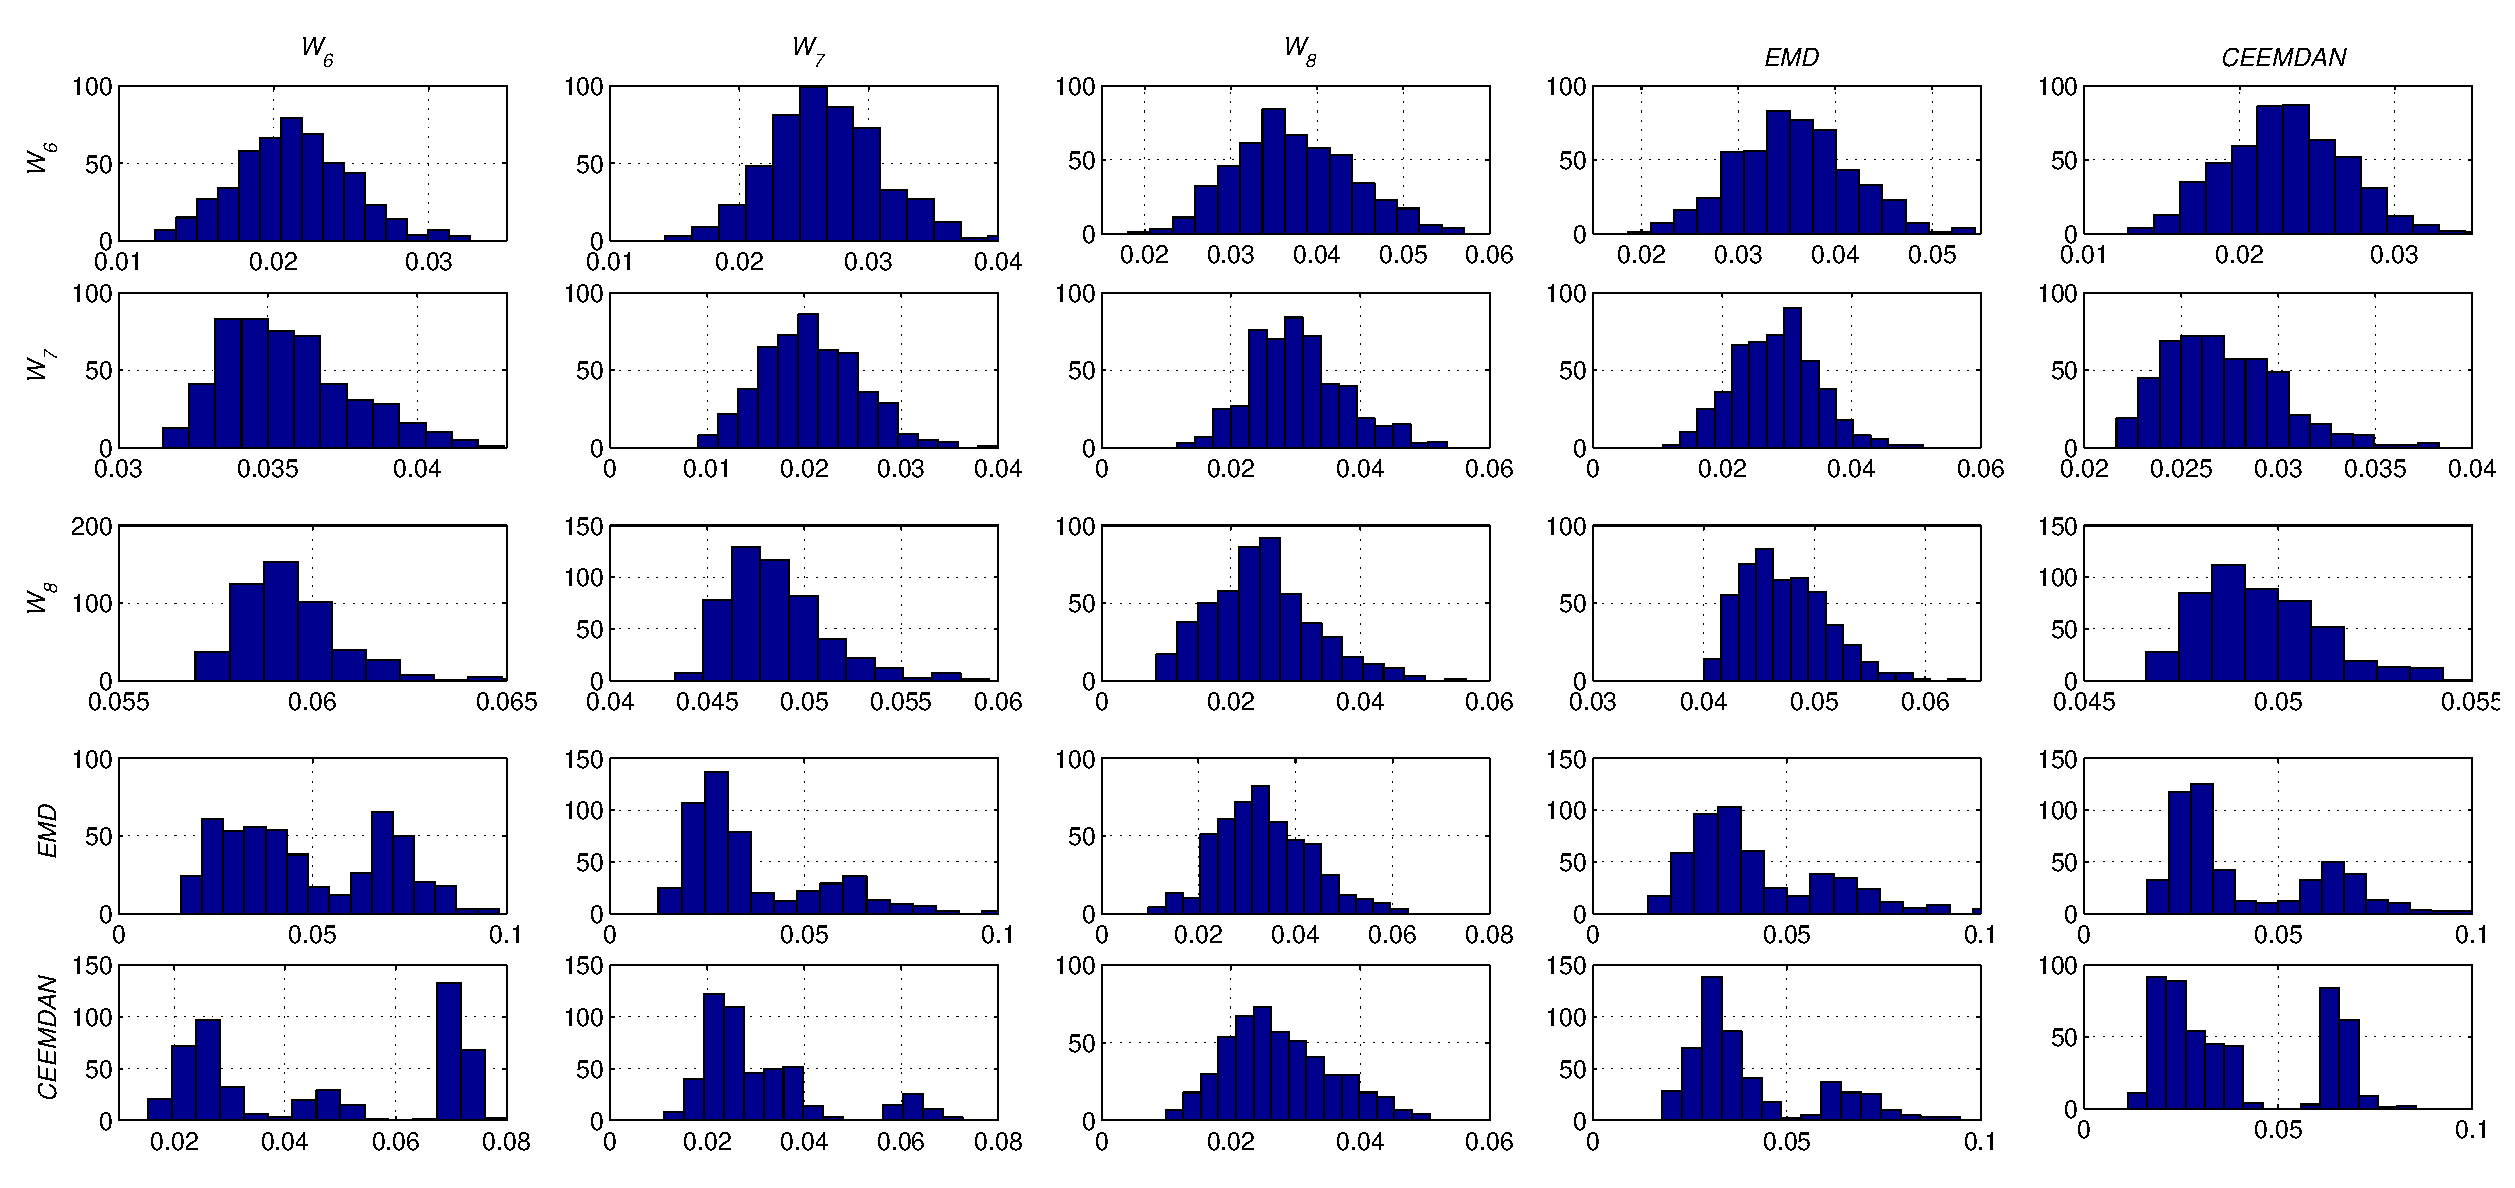
\includegraphics[width=1.0\textwidth,keepaspectratio]{Figure}
\caption{Название рисунка.}
\label{fig:}
\end{figure*}


% \appendix
% \section{Название приложения}
\label{sec:Appendix_}

Здесь размещается содержимое приложений к работе. В общем случае их может быть более одного.

\end{document}
